\pdfoutput=1

\documentclass{article}

% Use the following line for the initial blind version submitted for review:
% \usepackage{icml2025}

% If accepted, instead use the following line for the camera-ready submission:
\usepackage[accepted]{icml2025}

% Recommended, but optional, packages for figures and better typesetting:
\usepackage{microtype}
\usepackage{subfigure}
\usepackage{natbib}
% \setcitestyle{numbers,square}
% \setcitestyle{authoryear}


% generic packages
% \usepackage[left=1in, right=1in, top=1in, bottom=1in]{geometry}
\usepackage[utf8]{inputenc}
\usepackage{amsmath,amsfonts}
\usepackage{amssymb}
\usepackage{graphicx}
\usepackage{tikz}
\usepackage{mathtools}
\usepackage{amsthm}
\usepackage{nccmath}
\usepackage{xspace}
\usepackage{xcolor}
\usepackage{booktabs}
\usepackage{array}
\usepackage{subcaption}
\usepackage{mathrsfs}
\definecolor{MyBlue}{rgb}{0.12, 0.12, 0.76}
\definecolor{MyPurple}{rgb}{0.8, 0.1, 0.8}
\definecolor{MyGreen}{rgb}{0.7, 0.1, 0.1}
\definecolor{MyRed}{rgb}{0.8, 0.1, 0.3}
\definecolor{MyYellow}{rgb}{0.7, 0.7, .1}
\definecolor{MyBlue2}{rgb}{0.1, 0.1, 0.6}
\definecolor{Color3}{HTML}{D62728}
\definecolor{Color1}{HTML}{0050C8}
\definecolor{Color2}{HTML}{4DAF4A}
\usepackage[colorlinks,allcolors=black]{hyperref}
\usepackage{pifont}% http://ctan.org/pkg/pifont
\newcommand{\cmark}{\ding{51}}
\newcommand{\xmark}{\ding{55}}



\usepackage[group-separator={,}]{siunitx}
\usepackage{url}
\usepackage{enumitem}
\usepackage{pdflscape}
\usepackage{verbatim}
\usepackage{arydshln}
\usepackage{multirow}
\usepackage{bigdelim}
\usepackage{stfloats}
\usepackage{pgfplots}
\usepackage{cleveref}
% \usepackage[capitalize,noabbrev]{cleveref}
\usepackage[font=small]{caption}
\newsavebox{\taxonomy}


\usetikzlibrary{shadows,arrows,decorations,decorations.shapes,backgrounds,shapes,snakes,automata,fit,petri,shapes.multipart,calc,positioning,shapes.geometric,graphs,graphs.standard,plotmarks,math,arrows.meta}
\usepackage{tikz-qtree}

% so I can restate theorems
\usepackage{thmtools}
\usepackage{thm-restate}

% Theorems
\theoremstyle{plain}
\newtheorem{theorem}{Theorem}[section]
\newtheorem{proposition}[theorem]{Proposition}
\newtheorem{lemma}[theorem]{Lemma}
\newtheorem{corollary}{Corollary}[theorem]
% \theoremstyle{definition}
\newtheorem{definition}[theorem]{Definition}
\newtheorem{assumption}[theorem]{Assumption}
\theoremstyle{remark}
\newtheorem{remark}[theorem]{Remark}

% Restate with same number, different text
    \newtheoremstyle{TheoremNum}
        {\topsep}{\topsep}              %%% space between body and thm
        {\itshape}                      %%% Thm body font
        {}                              %%% Indent amount (empty = no indent)
        {\bfseries}                     %%% Thm head font
        {.}                             %%% Punctuation after thm head
        { }                             %%% Space after thm head
        {\thmname{#1}\thmnote{ \bfseries #3}}%%% Thm head spec
    \theoremstyle{TheoremNum}
    \newtheorem{theoremNumbered}{Theorem}





% To define a Construction environment
\usepackage{newfloat}
\DeclareFloatingEnvironment[
    fileext=los,
    listname={List of Constructions},
    name=Construction,
    placement=Htbhp,
]{construction}

%Pseudocode stuff
% \usepackage{algorithm}
% \usepackage{algpseudocode}
% \usepackage{algorithmicx}
% \renewcommand{\algorithmicforall}{\textbf{for each}} % ``for all'' -->``for each''
% \let\oldReturn\Return
% \renewcommand{\Return}{\state\oldReturn}
% \algtext*{EndWhile}% Remove "end while" text
% \algtext*{EndIf}
% \algtext*{EndForAll}
% \algtext*{EndFor}
% \algtext*{EndFunction}
\renewcommand{\algorithmicendfor}{\vspace{-1.2em}}%
\renewcommand{\algorithmicendif}{\vspace{-1.2em}}%

\DeclarePairedDelimiter{\ceil}{\lceil}{\rceil}
\DeclareMathOperator*{\argmax}{arg\,max}
\DeclareMathOperator*{\E}{\mathbb{E}}
\DeclareMathOperator*{\argmin}{arg\,min}
\DeclareMathOperator*{\len}{len}
\DeclareMathOperator*{\conv}{conv}
\DeclareMathOperator*{\vol}{vol}
\DeclareMathOperator*{\diam}{diam}


\newcommand\bbr{\mathbb{R}}
\newcommand\bbrpos{\mathbb{R}_{\ge 0}}
\newcommand\bbrspos{\mathbb{R}_{> 0}}
\newcommand\bbn{\mathbb{N}}
\newcommand\ep{\varepsilon}
\newcommand\hata{\hat{a}}
\renewcommand{\d}[1]{\ensuremath{\operatorname{d}\!{#1}}}
\newcommand\X{\mathcal{X}}
\newcommand\smola{\boldsymbol{a}}
\newcommand\smols{\boldsymbol{s}}
\newcommand\s{\mathcal{S}}
\newcommand\sm{\boldsymbol{s^m}}
\newcommand\A{\mathcal{A}}
\newcommand\bfone{\boldsymbol{1}}
\newcommand\norm[1]{||#1||}
\newcommand\tv[1]{||#1||_{TV}}
\newcommand\bfmu{\boldsymbol{\mu}}
\newcommand\muprime{\boldsymbol{\mu'}}
\newcommand\M{\mathcal{M}}
\newcommand\bars{\bar{s}}
\newcommand\rac{R_T^{AC}}
\newcommand{\spr}{\mathcal{S'}}
\newcommand{\mpr}{\mathcal{M'}}
\newcommand\apr{\mathcal{A'}}
\newcommand\U{\mathcal{U}}
\newcommand\tilpi{\tilde{\Pi}}
\newcommand\stilpi{\tilde{\pi}}
\newcommand\D{\mathcal{D}}
\newcommand\B{\mathcal{B}}

\newcommand\stuart[1]{{\color{purple}Stuart: #1}}
\newcommand\juan[1]{{\color{blue}Juan: #1}}
\newcommand\todo[1]{{\color{red}TODO: #1}}
% \renewcommand\todo[1]{}

% \title{Asking for Help Enables Safety Guarantees Without Sacrificing Effectiveness}

% \author{Benjamin Plaut\thanks{Corresponding author} \\
% UC Berkeley \\
% \texttt{plaut@berkeley.edu}
% \and Juan Liévano-Karim \\
% UC Berkeley \\
% \texttt{jp.lievano10@uniandes.edu.co}
% \and Stuart Russell \\
% UC Berkeley \\
% \texttt{russell@berkeley.edu}
% }

% \author{Anonymous authors}


\date{}

\icmltitlerunning{Asking for Help Enables Safety Guarantees Without Sacrificing Effectiveness}

\begin{document}

\twocolumn[
\icmltitle{Asking for Help Enables Safety Guarantees\\ Without Sacrificing Effectiveness}

% \maketitle

\icmlsetsymbol{equal}{*}

\begin{icmlauthorlist}
\icmlauthor{Benjamin Plaut}{ucb}
\icmlauthor{Juan Liévano-Karim}{ucb}
\icmlauthor{Stuart Russell}{ucb}
\end{icmlauthorlist}

\icmlaffiliation{ucb}{University of California, Berkeley}

\icmlcorrespondingauthor{Benjamin Plaut}{plaut@berkeley.edu}

% You may provide any keywords that you
% find helpful for describing your paper; these are used to populate
% the "keywords" metadata in the PDF but will not be shown in the document
\icmlkeywords{safe RL,asking for help,irreversibility,regret}

\vskip 0.3in
]

\printAffiliationsAndNotice{}

\begin{abstract}  
Test time scaling is currently one of the most active research areas that shows promise after training time scaling has reached its limits.
Deep-thinking (DT) models are a class of recurrent models that can perform easy-to-hard generalization by assigning more compute to harder test samples.
However, due to their inability to determine the complexity of a test sample, DT models have to use a large amount of computation for both easy and hard test samples.
Excessive test time computation is wasteful and can cause the ``overthinking'' problem where more test time computation leads to worse results.
In this paper, we introduce a test time training method for determining the optimal amount of computation needed for each sample during test time.
We also propose Conv-LiGRU, a novel recurrent architecture for efficient and robust visual reasoning. 
Extensive experiments demonstrate that Conv-LiGRU is more stable than DT, effectively mitigates the ``overthinking'' phenomenon, and achieves superior accuracy.
\end{abstract}  

\section{Introduction}


\begin{figure}[t]
\centering
\includegraphics[width=0.6\columnwidth]{figures/evaluation_desiderata_V5.pdf}
\vspace{-0.5cm}
\caption{\systemName is a platform for conducting realistic evaluations of code LLMs, collecting human preferences of coding models with real users, real tasks, and in realistic environments, aimed at addressing the limitations of existing evaluations.
}
\label{fig:motivation}
\end{figure}

\begin{figure*}[t]
\centering
\includegraphics[width=\textwidth]{figures/system_design_v2.png}
\caption{We introduce \systemName, a VSCode extension to collect human preferences of code directly in a developer's IDE. \systemName enables developers to use code completions from various models. The system comprises a) the interface in the user's IDE which presents paired completions to users (left), b) a sampling strategy that picks model pairs to reduce latency (right, top), and c) a prompting scheme that allows diverse LLMs to perform code completions with high fidelity.
Users can select between the top completion (green box) using \texttt{tab} or the bottom completion (blue box) using \texttt{shift+tab}.}
\label{fig:overview}
\end{figure*}

As model capabilities improve, large language models (LLMs) are increasingly integrated into user environments and workflows.
For example, software developers code with AI in integrated developer environments (IDEs)~\citep{peng2023impact}, doctors rely on notes generated through ambient listening~\citep{oberst2024science}, and lawyers consider case evidence identified by electronic discovery systems~\citep{yang2024beyond}.
Increasing deployment of models in productivity tools demands evaluation that more closely reflects real-world circumstances~\citep{hutchinson2022evaluation, saxon2024benchmarks, kapoor2024ai}.
While newer benchmarks and live platforms incorporate human feedback to capture real-world usage, they almost exclusively focus on evaluating LLMs in chat conversations~\citep{zheng2023judging,dubois2023alpacafarm,chiang2024chatbot, kirk2024the}.
Model evaluation must move beyond chat-based interactions and into specialized user environments.



 

In this work, we focus on evaluating LLM-based coding assistants. 
Despite the popularity of these tools---millions of developers use Github Copilot~\citep{Copilot}---existing
evaluations of the coding capabilities of new models exhibit multiple limitations (Figure~\ref{fig:motivation}, bottom).
Traditional ML benchmarks evaluate LLM capabilities by measuring how well a model can complete static, interview-style coding tasks~\citep{chen2021evaluating,austin2021program,jain2024livecodebench, white2024livebench} and lack \emph{real users}. 
User studies recruit real users to evaluate the effectiveness of LLMs as coding assistants, but are often limited to simple programming tasks as opposed to \emph{real tasks}~\citep{vaithilingam2022expectation,ross2023programmer, mozannar2024realhumaneval}.
Recent efforts to collect human feedback such as Chatbot Arena~\citep{chiang2024chatbot} are still removed from a \emph{realistic environment}, resulting in users and data that deviate from typical software development processes.
We introduce \systemName to address these limitations (Figure~\ref{fig:motivation}, top), and we describe our three main contributions below.


\textbf{We deploy \systemName in-the-wild to collect human preferences on code.} 
\systemName is a Visual Studio Code extension, collecting preferences directly in a developer's IDE within their actual workflow (Figure~\ref{fig:overview}).
\systemName provides developers with code completions, akin to the type of support provided by Github Copilot~\citep{Copilot}. 
Over the past 3 months, \systemName has served over~\completions suggestions from 10 state-of-the-art LLMs, 
gathering \sampleCount~votes from \userCount~users.
To collect user preferences,
\systemName presents a novel interface that shows users paired code completions from two different LLMs, which are determined based on a sampling strategy that aims to 
mitigate latency while preserving coverage across model comparisons.
Additionally, we devise a prompting scheme that allows a diverse set of models to perform code completions with high fidelity.
See Section~\ref{sec:system} and Section~\ref{sec:deployment} for details about system design and deployment respectively.



\textbf{We construct a leaderboard of user preferences and find notable differences from existing static benchmarks and human preference leaderboards.}
In general, we observe that smaller models seem to overperform in static benchmarks compared to our leaderboard, while performance among larger models is mixed (Section~\ref{sec:leaderboard_calculation}).
We attribute these differences to the fact that \systemName is exposed to users and tasks that differ drastically from code evaluations in the past. 
Our data spans 103 programming languages and 24 natural languages as well as a variety of real-world applications and code structures, while static benchmarks tend to focus on a specific programming and natural language and task (e.g. coding competition problems).
Additionally, while all of \systemName interactions contain code contexts and the majority involve infilling tasks, a much smaller fraction of Chatbot Arena's coding tasks contain code context, with infilling tasks appearing even more rarely. 
We analyze our data in depth in Section~\ref{subsec:comparison}.



\textbf{We derive new insights into user preferences of code by analyzing \systemName's diverse and distinct data distribution.}
We compare user preferences across different stratifications of input data (e.g., common versus rare languages) and observe which affect observed preferences most (Section~\ref{sec:analysis}).
For example, while user preferences stay relatively consistent across various programming languages, they differ drastically between different task categories (e.g. frontend/backend versus algorithm design).
We also observe variations in user preference due to different features related to code structure 
(e.g., context length and completion patterns).
We open-source \systemName and release a curated subset of code contexts.
Altogether, our results highlight the necessity of model evaluation in realistic and domain-specific settings.






\section{RELATED WORK}
\label{sec:relatedwork}
In this section, we describe the previous works related to our proposal, which are divided into two parts. In Section~\ref{sec:relatedwork_exoplanet}, we present a review of approaches based on machine learning techniques for the detection of planetary transit signals. Section~\ref{sec:relatedwork_attention} provides an account of the approaches based on attention mechanisms applied in Astronomy.\par

\subsection{Exoplanet detection}
\label{sec:relatedwork_exoplanet}
Machine learning methods have achieved great performance for the automatic selection of exoplanet transit signals. One of the earliest applications of machine learning is a model named Autovetter \citep{MCcauliff}, which is a random forest (RF) model based on characteristics derived from Kepler pipeline statistics to classify exoplanet and false positive signals. Then, other studies emerged that also used supervised learning. \cite{mislis2016sidra} also used a RF, but unlike the work by \citet{MCcauliff}, they used simulated light curves and a box least square \citep[BLS;][]{kovacs2002box}-based periodogram to search for transiting exoplanets. \citet{thompson2015machine} proposed a k-nearest neighbors model for Kepler data to determine if a given signal has similarity to known transits. Unsupervised learning techniques were also applied, such as self-organizing maps (SOM), proposed \citet{armstrong2016transit}; which implements an architecture to segment similar light curves. In the same way, \citet{armstrong2018automatic} developed a combination of supervised and unsupervised learning, including RF and SOM models. In general, these approaches require a previous phase of feature engineering for each light curve. \par

%DL is a modern data-driven technology that automatically extracts characteristics, and that has been successful in classification problems from a variety of application domains. The architecture relies on several layers of NNs of simple interconnected units and uses layers to build increasingly complex and useful features by means of linear and non-linear transformation. This family of models is capable of generating increasingly high-level representations \citep{lecun2015deep}.

The application of DL for exoplanetary signal detection has evolved rapidly in recent years and has become very popular in planetary science.  \citet{pearson2018} and \citet{zucker2018shallow} developed CNN-based algorithms that learn from synthetic data to search for exoplanets. Perhaps one of the most successful applications of the DL models in transit detection was that of \citet{Shallue_2018}; who, in collaboration with Google, proposed a CNN named AstroNet that recognizes exoplanet signals in real data from Kepler. AstroNet uses the training set of labelled TCEs from the Autovetter planet candidate catalog of Q1–Q17 data release 24 (DR24) of the Kepler mission \citep{catanzarite2015autovetter}. AstroNet analyses the data in two views: a ``global view'', and ``local view'' \citep{Shallue_2018}. \par


% The global view shows the characteristics of the light curve over an orbital period, and a local view shows the moment at occurring the transit in detail

%different = space-based

Based on AstroNet, researchers have modified the original AstroNet model to rank candidates from different surveys, specifically for Kepler and TESS missions. \citet{ansdell2018scientific} developed a CNN trained on Kepler data, and included for the first time the information on the centroids, showing that the model improves performance considerably. Then, \citet{osborn2020rapid} and \citet{yu2019identifying} also included the centroids information, but in addition, \citet{osborn2020rapid} included information of the stellar and transit parameters. Finally, \citet{rao2021nigraha} proposed a pipeline that includes a new ``half-phase'' view of the transit signal. This half-phase view represents a transit view with a different time and phase. The purpose of this view is to recover any possible secondary eclipse (the object hiding behind the disk of the primary star).


%last pipeline applies a procedure after the prediction of the model to obtain new candidates, this process is carried out through a series of steps that include the evaluation with Discovery and Validation of Exoplanets (DAVE) \citet{kostov2019discovery} that was adapted for the TESS telescope.\par
%



\subsection{Attention mechanisms in astronomy}
\label{sec:relatedwork_attention}
Despite the remarkable success of attention mechanisms in sequential data, few papers have exploited their advantages in astronomy. In particular, there are no models based on attention mechanisms for detecting planets. Below we present a summary of the main applications of this modeling approach to astronomy, based on two points of view; performance and interpretability of the model.\par
%Attention mechanisms have not yet been explored in all sub-areas of astronomy. However, recent works show a successful application of the mechanism.
%performance

The application of attention mechanisms has shown improvements in the performance of some regression and classification tasks compared to previous approaches. One of the first implementations of the attention mechanism was to find gravitational lenses proposed by \citet{thuruthipilly2021finding}. They designed 21 self-attention-based encoder models, where each model was trained separately with 18,000 simulated images, demonstrating that the model based on the Transformer has a better performance and uses fewer trainable parameters compared to CNN. A novel application was proposed by \citet{lin2021galaxy} for the morphological classification of galaxies, who used an architecture derived from the Transformer, named Vision Transformer (VIT) \citep{dosovitskiy2020image}. \citet{lin2021galaxy} demonstrated competitive results compared to CNNs. Another application with successful results was proposed by \citet{zerveas2021transformer}; which first proposed a transformer-based framework for learning unsupervised representations of multivariate time series. Their methodology takes advantage of unlabeled data to train an encoder and extract dense vector representations of time series. Subsequently, they evaluate the model for regression and classification tasks, demonstrating better performance than other state-of-the-art supervised methods, even with data sets with limited samples.

%interpretation
Regarding the interpretability of the model, a recent contribution that analyses the attention maps was presented by \citet{bowles20212}, which explored the use of group-equivariant self-attention for radio astronomy classification. Compared to other approaches, this model analysed the attention maps of the predictions and showed that the mechanism extracts the brightest spots and jets of the radio source more clearly. This indicates that attention maps for prediction interpretation could help experts see patterns that the human eye often misses. \par

In the field of variable stars, \citet{allam2021paying} employed the mechanism for classifying multivariate time series in variable stars. And additionally, \citet{allam2021paying} showed that the activation weights are accommodated according to the variation in brightness of the star, achieving a more interpretable model. And finally, related to the TESS telescope, \citet{morvan2022don} proposed a model that removes the noise from the light curves through the distribution of attention weights. \citet{morvan2022don} showed that the use of the attention mechanism is excellent for removing noise and outliers in time series datasets compared with other approaches. In addition, the use of attention maps allowed them to show the representations learned from the model. \par

Recent attention mechanism approaches in astronomy demonstrate comparable results with earlier approaches, such as CNNs. At the same time, they offer interpretability of their results, which allows a post-prediction analysis. \par



\section{Model}
\label{sec:model}
Let $[N] = \{1, 2, \dots, N \}$ be a set of $N$ agents.
We examine an environment in which a system interacts with the agents over $T$ rounds.
Every round $t\leq T$ comprises $N$ \emph{sessions}, each session represents an encounter of the system with exactly one agent, and each agent interacts exactly once with the system every round.
I.e., in each round $t$ the agents arrive sequentially. 


\paragraph{Arrival order} The \emph{arrival order} of round $t$, denoted as $\ordv_t=(\ord_t(1),\dots, \ord_t(N))$, is an element from set of all permutations of $[N]$. Each entry $q$ in $\ordv_t$ is the index of the agent that arrives in the $q^{\text{th}}$ session of round $t$.
For example, if $\ord_t(1) = 2$, then agent $2$ arrives in the first session of round $t$.
Correspondingly, $\ord_t^{-1}(i)=q$ implies that agent $i$ arrives in the $q^{\text{th}}$ session of round $t$. 

As we demonstrate later, the arrival order has an immediate impact on agent rewards. We call the mechanism by which the arrival order is set \emph{arrival function} and denote it by $\ordname$. Throughout the paper, we consider several arrival functions such as the \emph{uniform arrival} function, denoted by $\uniord$, and the \emph{nudged arrival} $\sugord$; we introduce those formally in Sections~\ref{sec:uniform} and~\ref{sec:nudge}, respectively.

%We elaborate more on this concept in Section~\ref{sec: arrival}.


\paragraph{Arms} We consider a set of $K \geq 2$ arms, $A = \{a_1, \ldots, a_K\}$. The reward of arm $a_i$ in round $t$ is a random variable $X_i^t \sim \mathcal{D}^t_i$, where the rewards $(X_i^t)_{i,t}$ are mutually independent and bounded within the interval $[0,1]$. The reward distribution $\mathcal{D}^t_i$ of arm $a_i$, $i\in [K]$ at round $t\in T$ is assumed to be non-stationary but independent across arms and rounds. We denote the realized reward of arm $a_i$ in round $t$ by $x_i^t$. We assume \emph{reward consistency}, meaning that rewards may vary between rounds but remain constant within the sessions of a single round. Specifically, if an arm $a_i$ is selected multiple times during round~$t$, each selection yields the same reward $x_i^t$, where the superscript $t$ indicates its dependence on the round rather than the session. This consistency enables the system to leverage information obtained from earlier sessions to make more informed decisions in later sessions within the same round. We provide further details on this principle in Subsection~\ref{subsec:information}.


\paragraph{Algorithms} An algorithm is a mapping from histories to actions. We typically expect algorithms to maximize some aggregated agent metric like social welfare. Let $\mathcal H^{t,q}$ denote the information observed during all sessions of rounds $1$ to $t-1$ and sessions $1$ to $q-1$ in round $t$.  The history $\mathcal H^{t,q}$ is an element from $(A \times [0,1])^{(t-1) \cdot N +q-1}$, consisting of pairs of the form (pulled arm, realized reward). Notice that we restrict our attention to \emph{anonymous} algorithms, i.e., algorithms that do not distinguish between agents based on their identities. Instead, they only respond to the history of arms pulled and rewards observed, without conditioning on which specific agent performed each action.
%In the most general case, algorithms make decisions at session $q$ of round $t$  based on the entire history $\mathcal H^{t,q}$ and the index of the arriving agent $\ord_t(q)$. %Furthermore, we sometimes assume that algorithms have Bayesian information, i.e., algorithms are aware of the distributions $(\mathcal D_i)^K_{i=1}$. 
Furthermore, we sometimes assume that algorithms have Bayesian information, meaning they are aware of the reward distributions $(\mathcal{D}^t_i)_{i,t}$. If such an assumption is required to derive a result, we make it explicit. %Otherwise, we do not assume any additional knowledge about the algorithm’s information. %This distinction allows us to analyze both general algorithms without prior distributional knowledge and specialized algorithms that leverage Bayesian information.


\paragraph{Rewards} Let $\rt{i}$ denote the reward received by agent $i \in [N]$ at round $t$, and let $\Rt{i}$ denote her cumulative reward at the end of round $t$, i.e., $\Rt{i} = \sum_{\tau=1}^{t}{r^{\tau}_{i}}$. We further denote the \emph{social welfare} as the sum of the rewards all agents receive after $T$ rounds. Formally, $\sw=\sum^{N}_{i=1}{R^T_i}$. We emphasize that social welfare is independent of the arrival order. 


\paragraph{Envy}
We denote by $\adift{i}{j}$ the reward discrepancy of agents $i$ and $j$ in round $t$; namely, $\adift{i}{j}= \rt{i} - \rt{j}$. %We call this term \omer{name??} reward discrepancy in round $t$. 
The (cumulative) \emph{envy} between two agents at round $t$ is the difference in their cumulative rewards. Formally, $\env_{i,j}^t= \Rt{i} - \Rt{j}$ is the envy after $t$ rounds between agent $i$ and $j$. We can also formulate envy as the sum of reward discrepancies, $\env_{i,j}^t= \sum^{t}_{\tau=1}{\adif{i}{j}^\tau}$. Notice that envy is a signed quantity and can be either positive or negative. Specifically, if $\env_{i,j}^t < 0$, we say that agent $i$ envies agent $j$, and if $\env_{i,j}^t > 0$, agent $j$ envies agent $i$. The main goal of this paper is to investigate the behavior of the \emph{maximal envy}, defined as
\[
\env^t = \max_{i,j \in [N]} \env^t_{i,j}.
\]
For clarity, the term \emph{envy} will refer to the maximal envy.\footnote{ We address alternative definitions of envy in Section~\ref{sec:discussion}.} % Envy can also be defined in alternative ways, such as by averaging pairwise envy across all agents. We address average envy in Section~\ref{sec:avg_envy}.}
Note that $\env_{i,j}^t$ are random variables that depend on the decision-making algorithm, realized rewards, and the arrival order, and therefore, so is $\env^t$. If a result we obtain regarding envy depends on the arrival order $\ordname$, we write $\env^t(\ordname)$. Similarly, to ease notation, if $\ordname$ can be understood from the context, it is omitted.



\paragraph{Further Notation} We use the subscript $(q)$ to address elements of the $q^{\text{th}}$ session, for $q\in [N]$.
That is, we use the notation $\rt{(q)}$ to denote the reward granted to the agent that arrives in the $q^{\text{th}}$ session of round $t$ and $\Rt{(q)}$ to denote her cumulative reward. %Additionally, we introduce the notation $\at{(q)}$ to denote the arm pulled in that session.
Correspondingly, $\sdift{q}{w} = \rt{(q)} - \rt{(w)}$ is the reward discrepancy of the agents arriving in the $q^{\text{th}}$ and $w^{\text{th}}$ sessions of round $t$, respectively. 
To distinguish agents, arms, sessions and rounds, we use the letters $i,j$ to mark agents and arms, $q,w$ for sessions, and $t,\tau$ for rounds.


\subsection{Example}
\label{sec: example}
To illustrate the proposed setting and notation, we present the following example, which serves as a running example throughout the paper.

\begin{table}[t]
\centering
\begin{tabular}{|c|c|c|c|}
\hline
$t$ (round) & $\ordv_t$ (arrival order) & $x_1^t$ & $x_2^t$ \\ \hline
1           & 2, 1                     & 0.6     & 0.92    \\ \hline
2           & 1, 2                     & 0.48    & 0.1     \\ \hline
3           & 2, 1                     & 0.15    & 0.8     \\ \hline
\end{tabular}
\caption{
    Data for Example~\ref{example 1}.
}
\label{tbl: example}
\end{table}

\begin{algorithm}[t]
\caption{Algorithm for Example~\ref{example 1}}
\label{alguni}
\DontPrintSemicolon 
\For{round $t = 1$ to $T$}{
    pull $a_{1}$ in the first session\label{alguniexample: first}\\
    \lIf{$x^t_1 \geq \frac{1}{2}$}{pull $a_{1}$ again in second session \label{alguniexample: pulling a again}}
    \lElse{pull $a_{2}$ in second session \label{alguniexample: sopt else}}
}
\end{algorithm}


\begin{example}\label{example 1}
We consider $K=2$ uniform arms, $X_1,X_2 \sim \uni{0,1}$, and $N=2$ for some $T\geq 3$. We shall assume arm decision are made by Algorithm~\ref{alguni}: In the first session, the algorithm pulls $a_1$; if it yields a reward greater than $\nicefrac{1}{2}$, the algorithm pulls it again in the second session (the ``if'' clause). Otherwise, it pulls $a_2$.



We further assume that the arrival orders and rewards are as specified in Table~\ref{tbl: example}. Specifically, agent 2 arrives in the first session of round $t=1$, and pulling arm $a_2$ in this round would yield a reward of $x^1_2 = 0.92$. Importantly, \emph{this information is not available to the decision-making algorithm in advance} and is only revealed when or if the corresponding arms are pulled.




In the first round, $\boldsymbol{\eta}^1 = \left(2,1\right)$; thus, agent 2 arrives in the first session.
The algorithm pulls arm $a_1$, which means, $a^1_{(1)} = a_1$, and the agent receives $r_{2}^1=r_{(1)}^1=x_1^1=0.6$.
Later that round, in the second session, agent 1 arrives, and the algorithm pulls the same arm again since $x^1_1 = 0.6 \geq \nicefrac{1}{2}$ due to the ``if'' clause.
I.e., $a^1_{(2)} = a_1$ and $r_{1}^1 = r_{(2)}^1 = x_1^1 = 0.6$.
Even though the realized reward of arm $a_2$ in that round is higher ($0.92$), the algorithm is not aware of that value.
At the end of the first round, $R^1_1 = R^1_{(2)} = R^1_2 = R^1_{(1)} = 0.6$. The reward discrepancy is thus $\adif{1}{2}^1 = \adif{2}{1}^1= \sdif{2}{1}^1 = 0.6 - 0.6 =0$. 



In the second round, agent 1 arrives first, followed by agent 2.
Firstly, the algorithm pulls arm $a_1$ and agent 1 receives a reward of $r_{1}^2 = r_{(1)}^2 = x_1^2 = 0.48$.
Because the reward is lower than $\nicefrac{1}{2}$, in the second session the algorithm pulls the other arm ($a^2_{(2)} = a_2$), granting agent 2 a reward of $r_{2}^2 = r_{(2)}^2 = x_2^2 = 0.1$.
At the end of the second round, $R^2_1 = R^2_{(1)} = 0.6 + 0.48 = 1.08$ and $R^2_2 = R^2_{(2)} = 0.6 + 0.1 = 0.7$. Furthermore, $\sdif{2}{1}^2 = \adif{2}{1}^2 = r^2_{2} - r^2_{1} = 0.1 - 0.48 = -0.38$.

In the third and final round, agent 2 arrives first again, and receives a reward  of $0.15$ from $a_1$. When agent 1 arrives in the second session, the algorithm pulls arm $a_2$, and she receives a reward of $0.8$. As for the reward discrepancy, $\sdif{2}{1}^3 = \adif{2}{1}^3 = r^3_{2} - r^3_{1} = 0.15 - 0.8 = -0.75$. 

Finally, agent 1 has a cumulative reward of $R^3_1 = R^3_{(2)} = 0.6 + 0.48 + 0.8 = 1.88$, whereas agent~2 has a cumulative reward of $R^3_2 = R^3_{(1)} = 0.6 + 0.1 + 0.15 = 0.85$. In terms of envy, $\env^1_{1,2}= \adif{1}{2}^1 =0$, $\env^2_{1,2}=\adif{1}{2}^1+\adif{1}{2}^2= 0.38$, and $\env^3_{1,2} = -\env^3_{2,1} = R^3_1-R^3_2 = 1.88-0.85 = 1.03$, and consequently the envy in round 3 is $\env^3 = 1.03$.
\end{example}


\subsection{Information Exploitation}
\label{subsec:information}

In this subsection, we explain how algorithms can exploit intra-round information.
Since rewards are consistent in the sessions of each round, acquiring information in each session can be used to increase the reward of the following sessions.
In other words, the earlier sessions can be used for exploration, and we generally expect agents arriving in later sessions to receive higher rewards.
Taken to the extreme, an agent that arrives after all arms have been pulled could potentially obtain the highest reward of that round, depending on how the algorithm operates.

To further demonstrate the advantage of late arrival, we reconsider Example~\ref{example 1} and Algorithm~\ref{alguni}. 
The expected reward for the agent in the first session of round $t$ is $\E{\rt{(1)}}=\mu_1=\frac{1}{2}$, yet the expected reward of the agent in the second session is
\begin{align*}
\E{\rt{(2)}}=\E{\rt{(2)}\mid X^t_1 \geq \frac{1}{2} }\prb{X^t_1 \geq \frac{1}{2}} + \E{\rt{(2)}\mid X^t_1 < \frac{1}{2} }\prb{X^t_1 < \frac{1}{2}};
\end{align*}
thus, $\E{\rt{(2)}} =\E{X^t_1\mid X^t_1 \geq \frac{1}{2} }\cdot \frac{1}{2} + \mu_2\cdot\frac{1}{2} = \frac{5}{8}$.
Consequently, the expected welfare per round is $\E{\rt{(1)}+\rt{(2)}}=1+\frac{1}{8}$, and the benefit of arriving in the second session of any round $t$ is $\E{\rt{(2)} - \rt{(1)}} = \frac{1}{8}$. This gap creates envy over time, which we aim to measure and understand.
%This discrepancy generates envy over time, and our paper aims to better understand it.
\subsection{Socially Optimal Algorithms}
\label{sec: sw}
Since our model is novel, particularly in its focus on the reward consistency element, studying social welfare maximizing algorithms represents an important extension of our work. While the primary focus of this paper is to analyze envy under minimal assumptions about algorithmic operations, we also make progress in the direction of social welfare optimization. See more details in Section~\ref{sec:discussion}.%Due to space limitations, we defer the discussion on socially optimal algorithms to  \ifnum\Includeappendix=0{the appendix}\else{Section~\ref{appendix:sociallyopt}}\fi.




% Since our model is novel and specifically the reward consistency element, it might be interesting to study social welfare optimization. While the main focus of our paper is to study envy under minimal assumptions on how the algorithm operates, we take steps toward this direction as well. Due to space limitations, we defer the discussion on socially optimal algorithms to  \ifnum\Includeappendix=0{the appendix}\else{Section~\ref{appendix:sociallyopt}}\fi.  We devise a socially optimal algorithm for the two-agent case, offer efficient and optimal algorithms for special cases of $N>2$ agents, and an inefficient and approximately optimal algorithm for any instance with $N>2$. Moreover, we address the welfare-envy tradeoff in Section~\ref{sec:extensions}.


% Social welfare, unlike envy, is entirely independent of the arrival order. While the main focus of our paper is to study envy under minimal assumptions on how the algorithm operates, socially optimal algorithms might also be of interest. Due to space limitations, we defer the discussion on socially optimal algorithms to  \ifnum\Includeappendix=0{the appendix}\else{Section~\ref{appendix:sociallyopt}}\fi. We devise a socially optimal algorithm for the two-agent case, offer efficient and optimal algorithms for special cases of $N>2$ agents, and an inefficient and approximately optimal algorithm for any instance with $N>2$. %Furthermore, we treat the welfare-envy tradeoff of the special case of Example~\ref{example 1}.





\begin{table*}[b!]
\centering
\caption{The key differences between our model and that of \citet{plaut_avoiding_2024}.}
\begin{tabular}{p{0.18\textwidth} p{0.36\textwidth} p{0.36\textwidth}}
\toprule
\textbf{Aspect} & \textbf{Our model} & \textbf{Model of \citet{plaut_avoiding_2024}} \\
\midrule
Conceptual goal & Maximize reward and avoid catastrophe & Avoid catastrophe only \\
% \midrule
% Reward meaning & Typical meaning & Chance of no catastrophe that round\\
\midrule
Objective & Sum of payoffs & Product of payoffs \\
\midrule
Regret definition & Agent and mentor evaluated on $\smols,\sm$ & Agent and mentor both evaluated on $\smols$ \\
\midrule
Desired regret & Sublinear in $T$ & Subconstant in $T$ \\
% \midrule
% Source of next state & MDP transition function & Adversary \\
% \midrule
% Smoothness & $\sigma$-smooth transition function & $\sigma$-smooth adversary \\
\bottomrule
\end{tabular}
\label{tab:model-comparison}
\end{table*}

\section{Avoiding catastrophe in \citet{plaut_avoiding_2024} and in MDPs}\label{sec:ac-overview}

Since our main result is a reduction to \citet{plaut_avoiding_2024}, we first describe their work. This section also serves to establish the novelty of our contribution in relation to \citet{plaut_avoiding_2024}. Some technical details are deferred to Appendix~\ref{sec:ac-full}.

Our model and that of \citet{plaut_avoiding_2024} are quite similar, so their model is perhaps best understood through comparison with our model. In place of $r$, they consider a sequence of reward functions $\bfmu = (\mu_1,\dots,\mu_T)$, where $\mu_t: \s\times\A\to[0,1]$ represents the probability of avoiding catastrophe at time $t$ (conditioned on no prior catastrophe). They aim to maximize the product of rewards from $\bfmu$, which is equal to the overall chance of avoiding catastrophe by the chain rule of probability. They also make a local generalization assumption: letting $\mu_t^m(s) = \mu_t(s, \pi^m(s))$ for brevity, we say that $\bfmu$ satisfies local generalization if $|\mu_t^m(s) - \mu_t(s, \pi^m(s'))| \le L\norm{s - s'}$ for all $s, s'\in \s$ and $t \in [T]$.


% \emph{Regret definition.} We evaluate the agent and mentor on their respective state sequences (as determined by their respective actions and the transition kernel). Instead, \citet{plaut_avoiding_2024} assume that a single state sequence is provided by an adversary\footnote{Their adversary can be adaptive: the choice of $s_t$ and $\mu_t$ can depend on the events of prior time steps.} and evaluate both the agent and the mentor on that same sequence. 

% \emph{Desired regret.} Instead of sublinear regret, \citet{plaut_avoiding_2024} demand \emph{subconstant} regret. That is, the total (not average) regret should go to 0 as $T \to\infty$. However, we will see that subconstant regret in their setting is of the same ``difficulty'' as sublinear regret in our setting (\Cref{sec:ac-mdp}).



\Cref{tab:model-comparison} summarizes the differences between our models. Formally, we arrive at \Cref{def:ac}:

\begin{restatable}{definition}{defAC}
\label{def:ac}
Let $\rac = \sup_{\M, \pi^m,\bfmu} \E[\sum_{t=1}^T \mu_t^m(s_t) - \sum_{t=1}^T \mu_t(s_t, a_t)]$, where the supremum ranges over all $\bfmu$ satisfying local generalization. Then an algorithm \emph{avoids catastrophe} if $Q_T \in o(T)$ and $\lim_{T\to\infty} \rac = 0$.\looseness=-1
\end{restatable}

\Cref{def:ac} was intended by \citet{plaut_avoiding_2024} to represent avoiding catastrophe. This interpretation can be debated, but ultimately we primarily use \Cref{def:ac} as a mathematical tool for our main goal: a no-regret algorithm for general MDPs. As such, what really matters is that \citet{plaut_avoiding_2024} give an algorithm satisfying \Cref{def:ac}.

% First, instead of evaluating the mentor on $\sm$ and the agent on $\smols$, \Cref{def:ac} evaluates both on $\smols$: this makes the problem easier. On the flip side, \Cref{def:ac} demands subconstant regret instead of sublinear regret, which makes the problem harder.  problem is not obviously easier or harder than our problem

% There are two subtleties in \Cref{def:ac}. 

Before stating the relevant lemma, we discuss two subtleties of \Cref{def:ac}. First, \citet{plaut_avoiding_2024} assume that the agent never observes $\mu_t(s_t,a_t)$ and only learns from mentor queries. Thus for fixed $\M$ and $\pi^m$, the choice of $\bfmu$ does not affect the behavior of the algorithm. As a result, \Cref{def:ac} in effect requires that for any $\M$ and $\pi^m$, the algorithm satisfies $\E[\sum_{t=1}^T \mu_t^m(s_t) - \sum_{t=1}^T \mu_t(s_t, a_t)] \le \rac$ \emph{simultaneously} for every $\bfmu$ satisfying local generalization. This enables us to use multiple choices of $\bfmu$ in our reduction.

Second, the reader may notice that \Cref{def:ac} involves the sum of rewards, while we stated previously that \citet{plaut_avoiding_2024} study the products of rewards. However, in this particular context, the sum and product formulations are roughly equivalent (\Cref{prop:sum-prod}).\footnote{This is mostly due to the approximation $1+x \approx e^x$ for $x \approx 0$.} Indeed, \citet{plaut_avoiding_2024} also include additive versions of all of their regret bounds. We use their additive bounds since those are more convenient for us. Specifically, they prove the following:\looseness=-1

% \footnote{Although \Cref{lem:ac-regret} assumes binary actions, \citet{plaut_avoiding_2024} also provide a version for any finite number of actions (Algorithm 3 and Theorem C.1 in their paper). Our result applies equally to that version -- indeed, our result is a general reduction -- but the many-action version requires more terminology to state, so we have chosen to only include the binary-action version here.}
\begin{lemma}[Theorems 5.2 and 5.3 in \citet{plaut_avoiding_2024}]
\label{lem:ac-regret}
    Let $\A = \{0,1\}$. Assume $\pi^m \in \Pi$ and either (1) $\Pi$ has finite VC dimension $d$ and $P$ is $\sigma$-smooth or (2) $\Pi$ has finite Littlestone dimension $d$.\footnote{The second case does not assume $\sigma$-smoothness, so the regret and query bounds in that case do not actually depend on $\sigma$. However, for brevity, we just write a single set of bounds.} Then Algorithm 1 in \citet{plaut_avoiding_2024} avoids catastrophe (\Cref{def:ac}) with
    % $Q_T \in  O(T^\frac{4n+1}{4n+2}(\frac{d}{\sigma} \log T + \diam(\smols)^n))$ and $\rac \in O(\frac{dL}{\sigma}T^\frac{-1}{2n+1} \log T)$.
\begin{align*}
Q_T \in&\  O\left(T^\frac{4n+1}{4n+2}\Big(\frac{d}{\sigma} \log T + \diam(\smols)^n\Big)\right)\\
\rac \in&\ O\left(\frac{dL}{\sigma}T^\frac{-1}{2n+1} \log T\right)
\end{align*}
\end{lemma}

Their algorithm has several beneficial properties beyond the regret and query bounds: it can handle an unbounded state space (the number of queries scales with the diameter of observed states), it does not need to know $L$, and it does not need to know how states are encoded in $\bbr^n$. See Appendix~\ref{sec:ac-full} for pseudocode for their algorithm.

Although \Cref{lem:ac-regret} requires $\A = \{0,1\}$, \citet{plaut_avoiding_2024} also provide a version for any finite number of actions (Algorithm 3 and Theorem C.1 in their paper). Our reduction applies equally to that version, but the many-action version requires more terminology to state, so we have chosen to only include the binary-action version here.


Lastly, although this does not directly bear on our results, it is worth mentioning that \citet{plaut_avoiding_2024} also prove a negative result: without the assumptions of \Cref{lem:ac-regret}, no algorithm satisfies both $Q_T \in o(T)$ and $\rac \in o(1)$, even for a simple environment: $\s = [0,1]$, i.i.d. states, and $\bfmu$ does not vary between time steps. We can expect this negative result to apply to our setting too, since obtaining high reward requires avoiding catastrophe. But what does ``catastrophe'' mean in an MDP?\looseness=-1

\textbf{Catastrophe in MDPs.} In contrast to the model of \citet{plaut_avoiding_2024}, MDPs do not directly model catastrophe in an objective function. Instead, notions of catastrophe arise naturally through the environment dynamics: for example, the agent might get stuck in an inescapable zero-reward state.\looseness=-1

\begin{figure*}[b]
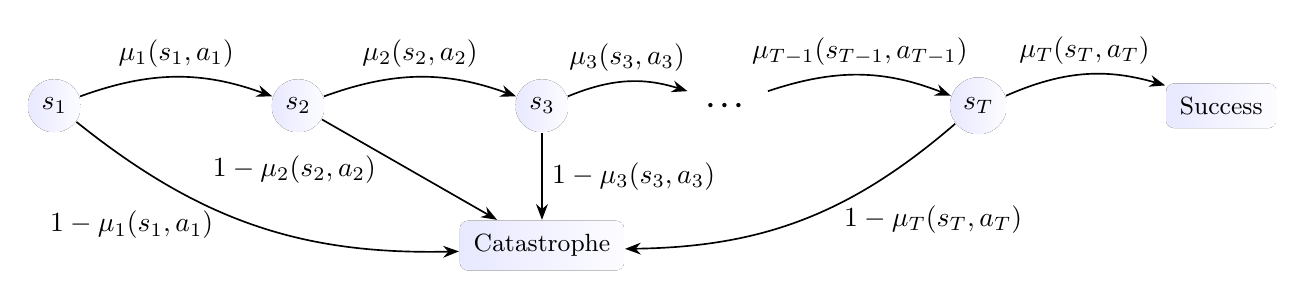
\begin{tikzpicture}[>={Stealth[scale=1]}, 
    semithick, 
    node distance=2.4cm, 
    auto, 
    state/.style={align=center,circle,inner sep=3pt,path picture={\fill[left color=blue!9, right color=blue!1] (path picture bounding box.south west) rectangle (path picture bounding box.north east);}}
    ]
    % Nodes
    \node[state] (S1) {$s_1$};
    \node[state, right=of S1] (S2) {$s_2$};
    \node[state, right=of S2] (S3) {$s_3$};
    \node[right=1.5cm of S3, minimum width=1 cm] (dots) {$\boldsymbol{\cdots}$};
    \node[state, right=2.3cm of dots] (ST) {$s_T$};
    \node[state, rectangle, rounded corners=3pt, below=1.1cm of S3, minimum width=1cm,inner sep=5pt] (TRAP) {\small Catastrophe};
        % \node[rectangle, rounded corners=3pt, path picture={\fill[left color=red!8, right color=red!2] (path picture bounding box.south west) rectangle (path picture bounding box.north east);}, below=1.4cm of S3, minimum width=1cm] (TRAP) {\small Catastrophe};
    \node[state, rectangle, rounded corners=3pt,right=2cm of ST, minimum width=1cm,inner sep=5pt] (SUCCESS) {\small Success};
    % \node[rectangle, rounded corners=3pt, path picture={\fill[left color=green!9, right color=green!3] (path picture bounding box.south west) rectangle (path picture bounding box.north east);},right=2cm of ST, minimum width=1cm] (SUCCESS) {\small Success};
    % Edges from S1
    \path[->] (S1) edge[bend left=20] node[midway, above] {$\mu_1(s_1, a_1)$} (S2);
    \path[->] (S1) edge[bend right=20] node[midway, left=.4cm] {$1 - \mu_1(s_1, a_1)$} (TRAP);
    % Edges from S2
    \path[->] (S2) edge[bend left=20] node[midway, above] {$\mu_2(s_2, a_2)$} (S3);
    \path[->] (S2) edge node[midway, left=.3 cm] {$1 - \mu_2(s_2, a_2)$} (TRAP);
    % Edges from S3
    \path[->] (S3) edge[bend left=20] node[midway, above] {$\mu_3(s_3, a_3)$} (dots);
    \path[->] (S3) edge node[midway, right] {$1 - \mu_3(s_3, a_3)$} (TRAP);
    % Edge from dots
    \path[->] (dots) edge[bend left=20] node[midway,above] {$\mu_{T-1}(s_{T-1}, a_{T-1})$} (ST);
    % Edges from ST
    \path[->] (ST) edge[bend left=20] node[midway, above] {$\mu_T(s_T, a_T)$} (SUCCESS);
    \path[->] (ST) edge[bend left=20] node[midway, right=.4 cm] {$1 - \mu_T(s_T, a_T)$} (TRAP);
\end{tikzpicture}
\caption{An MDP where the only goal is to avoid catastrophe. On each time step $t$, the agent avoids catastrophe with probability $\mu_t(s_t, a_t)$, and otherwise transitions to a catastrophe state. If the agent avoids catastrophe for $T$ time steps, it reaches a success state. Suppose the agent receives reward $T$ upon reaching the success state and reward 0 elsewhere. (To keep rewards in $[0,1]$, one can double the time horizon so the agent spends $T$ time steps in the success state.) Then the agent's regret is  $R_T(\M, \pi^m) = T \cdot \E\big[\prod_{t=1}^T \mu_t^m(s_t)- \prod_{t=1}^T \mu_t(s_t, a_t)\big]$. Thus $R_T(\M, \pi^m) \in o(T)$ if and only if $\lim_{T\to\infty} \E\big[\prod_{t=1}^T \mu_t^m(s_t)- \prod_{t=1}^T \mu_t(s_t, a_t)\big] = 0$. In other words, the agent obtains \emph{sublinear} regret in the MDP iff it obtains \emph{subconstant} regret with respect to $\bfmu$.}
\label{fig:trap}
\end{figure*}

To be concrete, consider the MDP in \Cref{fig:trap}. An agent obtains sublinear regret in this MDP iff it obtains subconstant regret with respect to $\bfmu$: in particular, both occur iff the agent reaches the success state. This means that on a technical level, avoiding catastrophe in an MDP and avoiding catastrophe in the sense of \citet{plaut_avoiding_2024} are the same ``difficulty''. However, on top of avoiding catastrophe, we expect the agent to obtain high reward. Framed differently,  \citet{plaut_avoiding_2024} only consider the simple class of MDPs in \Cref{fig:trap}, while we prove that their algorithm performs well across all MDPs.


\begin{table*}[t]
\resizebox{\textwidth}{!}{
\begin{tabular}{cccccccccccc}
\hline
\multirow{2}{*}{$\alpha$} & \multirow{2}{*}{Method} & \multicolumn{5}{c}{$\beta = 0.2$}                                                                                                         & \multicolumn{5}{c}{$\beta = 0.4$}                                                                                     \\ \cline{3-12} 
                          &                         & Precision                 & Recall                    & F1                        & Accuracy                  & AUC                       & Precision             & Recall                & F1                    & Accuracy              & AUC                   \\ \hline
\multirow{7}{*}{0.2}      & FedAvg                  & 53.94 $\pm$ 3.56          & 54.05 $\pm$ 3.53          & 53.21 $\pm$ 3.90          & 53.41 $\pm$ 3.71          & 69.39 $\pm$ 2.05          & 53.58 $\pm$ 2.34      & 53.80 $\pm$ 2.77      & 52.30 $\pm$ 2.32      & 52.64 $\pm$ 2.14      & 68.20 $\pm$ 2.72      \\
                          & FedProx                 & 55.81 $\pm$ 1.58          & 54.37 $\pm$ 5.19          & 54.32 $\pm$ 2.21          & 54.62 $\pm$ 2.18          & 68.29 $\pm$ 2.93          & 54.39 $\pm$ 2.69      & 54.36 $\pm$ 1.82      & 53.27 $\pm$ 2.99      & 53.52 $\pm$ 2.97      & 68.11 $\pm$ 2.74      \\
                          & FedMed-GAN              & 54.62 $\pm$ 1.02          & 55.18 $\pm$ 2.73          & 53.46 $\pm$ 0.97          & 53.52 $\pm$ 1.07          & 68.80 $\pm$ 2.16          & 53.87 $\pm$ 3.66      & 54.66 $\pm$ 3.57      & 53.35 $\pm$ 3.61      & 53.41 $\pm$ 3.63      & 68.09 $\pm$ 2.53      \\
                          & FedMI                   & 54.77 $\pm$ 2.94          & 55.22 $\pm$ 4.36          & 54.26 $\pm$ 2.82          & 54.40 $\pm$ 2.83          & 69.15 $\pm$ 2.73          & 54.03 $\pm$ 3.88      & 54.46 $\pm$ 3.56      & 53.54 $\pm$ 4.22      & 53.63 $\pm$ 4.14      & 67.61 $\pm$ 3.93      \\
                          & MFCPL                   & 54.54 $\pm$ 1.88          & \textbf{56.06 $\pm$ 4.14} & 53.88 $\pm$ 1.64          & 54.07 $\pm$ 1.93          & 69.39 $\pm$ 2.71          & 53.86 $\pm$ 5.42      & 54.01 $\pm$ 5.44      & 53.22 $\pm$ 5.16      & 53.30 $\pm$ 5.34      & 67.58 $\pm$ 3.67      \\
                          & PmcmFL                  & 53.17 $\pm$ 1.60          & 52.73 $\pm$ 3.50          & 52.58 $\pm$ 1.81          & 52.64 $\pm$ 2.03          & 67.51 $\pm$ 4.07          & 49.03 $\pm$ 1.55      & 48.01 $\pm$ 3.03      & 48.38 $\pm$ 2.00      & 48.46 $\pm$ 2.31      & 63.71 $\pm$ 2.50      \\
                          & ClusMFL                    & \textbf{57.16 $\pm$ 2.32}     & 54.73 $\pm$ 3.93              & \textbf{56.56 $\pm$ 2.36}     & \textbf{56.92 $\pm$ 2.41}     & \textbf{72.81 $\pm$ 3.64}     & \textbf{56.06 $\pm$ 1.31} & \textbf{55.44 $\pm$ 2.19} & \textbf{55.38 $\pm$ 1.07} & \textbf{55.49 $\pm$ 1.10} & \textbf{72.50 $\pm$ 2.02} \\ \hline
\multirow{7}{*}{0.4}      & FedAvg                  & 53.75 $\pm$ 3.86          & 54.26 $\pm$ 3.76          & 52.76 $\pm$ 4.64          & 53.08 $\pm$ 4.34          & 67.91 $\pm$ 3.48          & 52.60 $\pm$ 3.00      & 53.95 $\pm$ 3.66      & 51.84 $\pm$ 3.06      & 51.98 $\pm$ 3.07      & 67.03 $\pm$ 3.22      \\
                          & FedProx                 & 54.36 $\pm$ 3.50          & 54.28 $\pm$ 4.17          & 53.77 $\pm$ 3.48          & 53.96 $\pm$ 3.51          & 68.26 $\pm$ 3.53          & 52.16 $\pm$ 2.20      & 52.93 $\pm$ 3.76      & 51.35 $\pm$ 2.13      & 51.54 $\pm$ 2.07      & 67.43 $\pm$ 3.64      \\
                          & FedMed-GAN              & 52.97 $\pm$ 1.63          & 52.89 $\pm$ 2.41          & 52.43 $\pm$ 1.74          & 52.53 $\pm$ 1.63          & 67.25 $\pm$ 3.45          & 53.56 $\pm$ 3.57      & 54.02 $\pm$ 3.95      & 52.54 $\pm$ 3.97      & 52.86 $\pm$ 3.63      & 67.91 $\pm$ 2.93      \\
                          & FedMI                   & 55.40 $\pm$ 2.85          & 53.82 $\pm$ 2.45          & 54.84 $\pm$ 2.75          & 54.95 $\pm$ 2.69          & 68.59 $\pm$ 2.48          & 54.01 $\pm$ 2.07      & 52.36 $\pm$ 1.98      & 53.62 $\pm$ 2.14      & 53.85 $\pm$ 2.06      & 66.70 $\pm$ 2.63      \\
                          & MFCPL                   & 55.07 $\pm$ 4.34          & 54.66 $\pm$ 3.93          & 54.34 $\pm$ 4.37          & 54.51 $\pm$ 4.57          & 66.60 $\pm$ 2.58          & 52.84 $\pm$ 4.14      & 54.69 $\pm$ 3.92      & 51.70 $\pm$ 3.89      & 51.87 $\pm$ 3.74      & 67.81 $\pm$ 3.48      \\
                          & PmcmFL                  & 51.71 $\pm$ 5.54          & 49.80 $\pm$ 6.21          & 50.77 $\pm$ 5.21          & 50.88 $\pm$ 5.42          & 65.54 $\pm$ 6.22          & 52.45 $\pm$ 3.96      & 50.03 $\pm$ 5.74      & 50.40 $\pm$ 4.72      & 50.77 $\pm$ 4.66      & 63.31 $\pm$ 5.17      \\
                          & ClusMFL                    & \textbf{56.59 $\pm$ 4.53} & \textbf{54.68 $\pm$ 4.49} & \textbf{56.17 $\pm$ 4.08} & \textbf{56.37 $\pm$ 4.10} & \textbf{73.25 $\pm$ 4.11} & \textbf{54.83 $\pm$ 6.13} & \textbf{54.88 $\pm$ 6.09} & \textbf{54.22 $\pm$ 5.89} & \textbf{54.40 $\pm$ 6.03} & \textbf{72.22 $\pm$ 4.47} \\ \hline
\end{tabular}
}
\caption{Performance Comparison Across Different Federated Learning Methods (Mean $\pm$ Standard Deviation \%) under Different Settings.}
\label{main result}
\end{table*}


% \input{proof_with_explanation}

\subsection{Proof sketch}

\begin{figure*}
\resizebox{\linewidth}{!}{
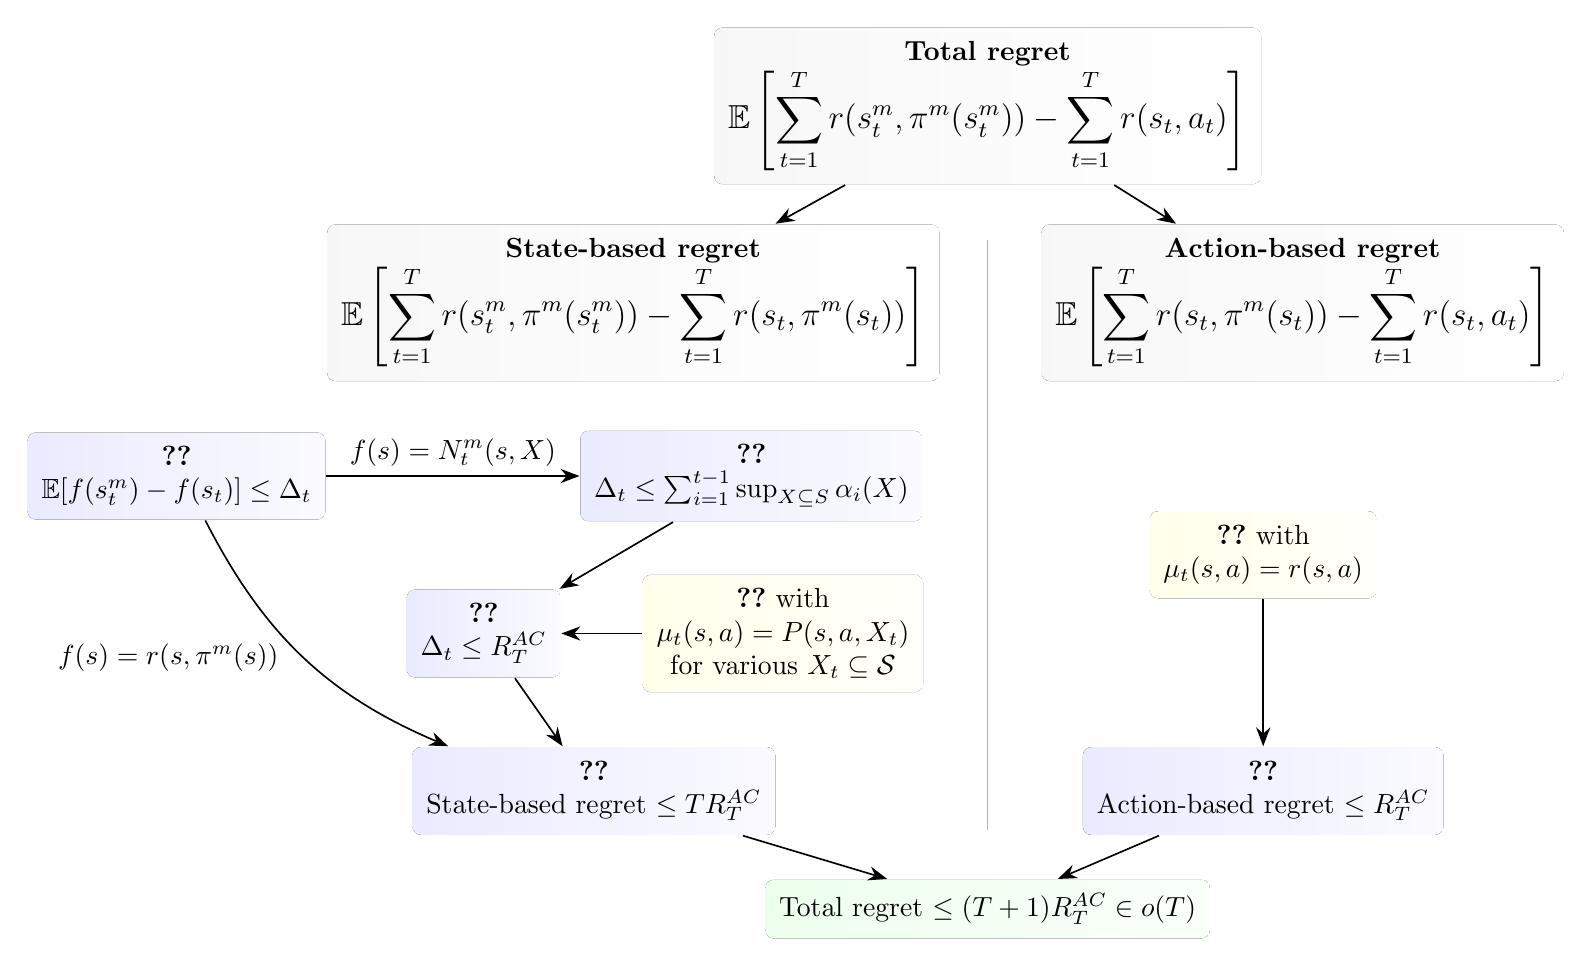
\begin{tikzpicture}[
>={Stealth[scale=1.2]}, 
    semithick, 
    group/.style={align=center,rounded corners=3pt,inner sep=5pt,path picture={\fill[left color=black!3, right color=black!0] (path picture bounding box.south west) rectangle (path picture bounding box.north east);}},
    lemma/.style={rounded corners=3pt, align=center,inner sep=5 pt,path picture={\fill[left color=blue!8, right color=blue!2] (path picture bounding box.south west) rectangle (path picture bounding box.north east);}},
    def/.style={rounded corners=3pt, align=center,inner sep=5 pt,        path picture={\fill[left color=yellow!8, right color=yellow!2] (path picture bounding box.south west) rectangle (path picture bounding box.north east);}},
    arrow/.style={->}
    % path picture={\fill[left color=red!10, right color=red!3] (path picture bounding box.south west) rectangle (path picture bounding box.north east);}]
    % path picture={\fill[left color=red!10, right color=red!3] (path picture bounding box.south west) rectangle (path picture bounding box.north east);}]
]
% Main decomposition
\node[group] (total) at (0,.7) {\textbf{Total regret}\\\large$\displaystyle \E\left[\sum_{t=1}^T r(s_t^m, \pi^m(s_t^m)) - \sum_{t=1}^T r(s_t, a_t)\right]$};

\node[group] (state) at (-4.5,-1.8) {\textbf{State-based regret}\\\large$\displaystyle \E\left[\sum_{t=1}^T r(s_t^m, \pi^m(s_t^m)) - \sum_{t=1}^T r(s_t, \pi^m(s_t))\right]$};

\node[group] (action) at (4,-1.8) {\textbf{Action-based regret}\\\large$\displaystyle \E\left[\sum_{t=1}^T r(s_t, \pi^m(s_t)) - \sum_{t=1}^T r(s_t, a_t)\right]$};

% State-based analysis
    \node[lemma] (lemma54) at (-10.3,-4) {\emph{\Cref{lem:split}} \\$\E[f(s_t^m) - f(s_t)] \leq \Delta_t$};

\node[lemma] (lemma55) at (-3,-4) {\emph{\Cref{lem:trajectories-induction}}\\$\Delta_t \leq \sum_{i=1}^{t-1} \sup_{X \subseteq S} \alpha_i(X)$};

\node[def] (defn41_x) at (-2.6,-6) {\Cref{def:ac} with\\$\mu_t(s,a) = P(s,a,X_t)$\\ for various $X_t\subseteq \s$};

\node[lemma] (lemma56) at (-6.4,-6) {\emph{\Cref{lem:trajectories}}\\$\Delta_t \leq R_T^{AC}$};

% \node[rounded corners=3pt, align=center,inner sep=5 pt] (interm) at (-10.6,-7.1) {$\E[r(s_t^m, \pi^m(s_t^m)) - r(s_t,\pi^m(s_t))] \le \Delta_t$};

\node[lemma] (statefinal) at (-5, -8) {\emph{\Cref{lem:state-regret}}\\ State-based regret $\le T R_T^{AC}$};

% \node[lemma] (statedelta) at (-10.5,-6.1) {$E[r(s_t^m, \pi^m(s_t^m)) - r(s_t, \pi^m(s_t))] \le \Delta_t$};

% Action-based analysis
\node[def] (defn41) at (3.5,-5) {\Cref{def:ac} with\\ $\mu_t(s,a) = r(s,a)$};

\node[lemma] (lemma53) at (3.5,-8) {\emph{\Cref{lem:action-regret}}\\Action-based regret $\leq R_T^{AC}$};

% Final result
\node[group,path picture={\fill[left color=green!7, right color=green!2] (path picture bounding box.south west) rectangle (path picture bounding box.north east);}] (final) at (0,-9.5) {Total regret $\leq (T+1)R_T^{AC} \in o(T)$};

% Main decomposition arrows
\draw[arrow] (total) -- (state);
\draw[arrow] (total) -- (action);

% State-based lemma dependency arrows
\draw[arrow] (lemma54) -- (lemma55) node[above,midway] {$f(s) = N_t^m(s,X)$};
\draw[arrow] (lemma55) -- (lemma56);
\draw[arrow] (defn41_x) -- (lemma56);
\draw[arrow] (lemma56) to (statefinal);
% \draw[arrow] (lemma54) -- (statedelta) node[midway,left] {$f(s) = r(s,\pi^m(s))$};
\draw[arrow] (lemma54) to[bend right=20] node[midway,left=.2cm] {$f(s) = r(s,\pi^m(s))$} (statefinal);
% \draw[arrow] (lemma54) to[bend right=20] (statefinal);
% \draw[arrow] (statedelta) to[bend right=20] (statefinal);
\draw[arrow] (statefinal) -- (final);
\draw[-,draw=black!30] (0,-1) -- (0,-8.5);

% Action-based arrows
\draw[arrow] (defn41) -- (lemma53);
\draw[arrow] (lemma53) -- (final);

\end{tikzpicture}
}
\caption{We decompose regret into state-based and action-based components by adding and subtracting $\E\big[\sum_{t=1}^T r(s_t,\pi^m(s_t))\big]$. Below, we show the dependencies of lemmas and applications of \Cref{def:ac} in the proof, leading to the final bound of $R_T \le (T+1)\rac$.}
\label{fig:proof}
\end{figure*}

The full proof is deferred to Appendix~\ref{sec:main-proof}, but we provide a visualization (\Cref{fig:proof}) and proof sketch here. 

First, we bound the action-based regret by a direct application of \Cref{def:ac}.\footnote{The fact that bounding the action-based regret is so simple is more a property of \Cref{def:ac} than of the decomposition.}

\begin{restatable}{lemma}{lemActionRegret}
\label{lem:action-regret}
If an algorithm satisfies \Cref{def:ac}, then $\E \big[\sum_{t=1}^T r(s_t, \pi^m(s_t)) - \sum_{t=1}^Tr(s_t, a_t)\big] \le  \rac$.
\end{restatable}

\begin{proof}
Let $\mu_t(s,a) := r(s,a)$ for all $t \in [T]$. Since $r$ satisfies local generalization, so does $\bfmu$. Hence by  \Cref{def:ac}, $\E \big[\sum_{t=1}^T r(s_t, \pi^m(s_t)) - \sum_{t=1}^T r(s_t, a_t)\big] \le  \rac$.
\end{proof}

It remains to bound the state-based regret. Rather than analyzing when $\smols$ is better or worse than $\sm$, we simply bound how much their distributions differ at all. Specifically, we will show that $\sup_{X\subseteq \s}(p_t^m(X) - p_t(X)) \le \rac$ for all $t \in [T]$. Let $\Delta_t = \sup_{X\subseteq \s}(p_t^m(X) - p_t(X))$; we will refer to this quantity frequently. 
First, we show that an entire class of expected values can be bounded by $\Delta_t$.


\begin{restatable}{lemma}{lemSplit}
\label{lem:split}
For any $t \in [T]$ and any measurable function $f: \s \to [0,1]$,  we have $\E[f(s_t^m) - f(s_t)] \le \Delta_t$.
\end{restatable}

The idea behind \Cref{lem:split} is that $\E[f(s_t^m) - f(s_t)]$ can only be large if $s_t^m$ is more concentrated than $s_t$ in states where $f$ is large. We use $\Delta_t$ to measure how large that difference in concentration can be. Also, since $f(s) \in [0,1]$, $f$ cannot be too much larger in these states where $s_t^m$ is more concentrated than $s_t$. Although there are some technical details, conceptually the proof amounts to:
\begin{align*}
\E[f(s_t^m) - f(s_t)] \le \sup_{s,s' \in \s} |f(s) - f(s')|\cdot  \Delta_t
\le  \Delta_t
\end{align*}
The most obvious application of \Cref{lem:split} is with $f(s) = r(s, \pi^m(s))$, and indeed, that will be one usage. However, we will also use this lemma to analyze the divergence between $\smols$ and $\sm$. Specifically, we will write $p_{t+1}^m(X) - p_{t+1}(X) = \E[f(s_t^m) - f(s_t)] + \alpha_t(X)$ for some functions $f$ and $\alpha_t$. Then \Cref{lem:split} will imply that
\begin{align*}
p_{t+1}^m(X) - p_{t+1}(X) \le&\ \Delta_t + \alpha_t(X) \quad \text{$\forall X \subseteq \s$}\\
\sup_{X\subseteq \s} (p_{t+1}^m(X) - p_{t+1}(X)) \le&\ \Delta_t + \sup_{X\subseteq \s} \alpha_t(X)\\
\Delta_{t+1} \le&\ \Delta_t + \sup_{X\subseteq \s} \alpha_t(X)
\end{align*}
The agent and mentor have the same initial state, so $\Delta_1 = 0$ and thus $\Delta_t \le \sum_{i=1}^{t-1} \sup_{X\subseteq \s} \alpha_t(X)$ by induction.

To enact this plan, we choose $f(s) = N_t^m(s,X)$ and $\alpha_t(X) = \E[N_t^m(s_t, X) - N_t(s_t, X)]$. Recall from \Cref{sec:model} that $N_t^m(s, X) = \Pr[s_{t+1}^m \in X \mid s_t^m = s]$ and $N_t(s,X) = \Pr[s_{t+1} \in X \mid s_t = s]$. The law of total expectation implies that $p_{t+1}^m(X) = \E[N_t^m(s_t^m, X)]$ and $p_{t+1}(X) = \E[N_t(s_t, X)]$, so
\begin{align*}
& \ \ p_{t+1}^m(X) - p_{t+1}(X)\\
=&\ \E[N_t^m(s_t^m, X)] - \E[N_t(s_t, X)]\\
=&\ \resizebox{\linewidth}{!}{%
\(\E[N_t^m(s_t^m, X) - N_t^m(s_t, X)] + \E[N_t^m(s_t, X) - N_t(s_t, X)]\)
}
\\
=&\ \E[N_t^m(s_t^m, X) - N_t^m(s_t, X)] + \alpha_t(X)
\end{align*}
(Interestingly, this decomposition is similar in structure to the state- vs action-based regret decomposition, although the terms here do not depend on $r$ at all.) 

This decomposition allows us to apply the aforementioned inductive strategy to obtain the following lemma:

\begin{restatable}{lemma}{lemTrajInd}\label{lem:trajectories-induction}
For any $t \in [T]$, $\Delta_t \le \sum_{i=1}^{t-1}\sup_{X\subseteq \s}\alpha_i(X)$.
\end{restatable}

This brings us to the trickiest part of the proof: bounding $\sum_{i=1}^{t-1}\sup_{X\subseteq \s}\alpha_i(X)$. The main idea is to invoke \Cref{def:ac} with $\mu_i(s, a) = P(s,a,X_i)$ for each $i \in [t-1]$ for every possible choice of $X_1,\dots,X_{t-1} \subseteq \s$. (It is also helpful to define $\mu_i(s,a)$ to be constant for $i > t$.) 

One can use the definition of total variation distance to show that if $P$ satisfies local generalization, so does this definition of $\bfmu$. Next, we can manipulate conditional expectations to show that $\E[N_i(s_i,X_i)] = \E[P(s_i,a_i,X_i)] = \E[\mu_i(s_i,a_i)]$ and $\E[N_i^m(s_i, X_i)] = \E[P(s_i, \pi^m(s_i), X_i)] = \E[\mu_i^m(s_i)]$. Thus applying \Cref{def:ac} to \Cref{lem:trajectories-induction} gives us
\begin{align*}
\Delta_t \le \sum_{i=1}^{t-1}\alpha_i(X_i) 
= \sum_{i=1}^T \E[\mu_i^m(s_i) - \mu_i(s_i, a_i)]
\le R_T^{AC}
\end{align*}
The result is \Cref{lem:trajectories}:

\begin{restatable}{lemma}{lemTraj}
\label{lem:trajectories}
If an algorithm satisfies \Cref{def:ac}, then $\Delta_t \le \rac$ for all $t \in [T]$.
\end{restatable}

Now we can bound the state-based regret by applying \Cref{lem:split} with $f(s) = r(s, \pi^m(s))$ followed by \Cref{lem:trajectories}. Specifically, we obtain
\[
\E\big[r(s_t^m, \pi^m(s_t^m)) - r(s_t, \pi^m(s_t))\big] \le \Delta_t \le \rac
\]
Summing this over $t$ produces \Cref{lem:state-regret}:

\begin{restatable}{lemma}{lemStateRegret}
\label{lem:state-regret}
If an algorithm satisfies \Cref{def:ac}, then \resizebox{1.02\linewidth}{!}{%
$\E\big[\sum_{t=1}^T r(s_t^m, \pi^m(s_t^m)) - \sum_{t=1}^T r(s_t, \pi^m(s_t))\big] \le T \rac$
.}
\end{restatable}

Since the state-based regret is at most $T \rac$ (\Cref{lem:state-regret}) and the action-based regret is at most $\rac$ (\Cref{lem:action-regret}), we conclude that $R_T \le (T+1)\rac$.

\section{Conclusion}
In this work, we propose a simple yet effective approach, called SMILE, for graph few-shot learning with fewer tasks. Specifically, we introduce a novel dual-level mixup strategy, including within-task and across-task mixup, for enriching the diversity of nodes within each task and the diversity of tasks. Also, we incorporate the degree-based prior information to learn expressive node embeddings. Theoretically, we prove that SMILE effectively enhances the model's generalization performance. Empirically, we conduct extensive experiments on multiple benchmarks and the results suggest that SMILE significantly outperforms other baselines, including both in-domain and cross-domain few-shot settings.

\section*{Impact statement}

In recent years, AI systems have grown increasingly capable and pervasive. Given this, we believe that safety guarantees for such systems are paramount. We are particularly concerned about harms that cannot be undone, which is the focus of the present paper. We hope that our work demonstrates that safety and effectiveness need not be at odds and can actually be simultaneously achieved. We have not identified any specific risks from our work that warrant special attention.

\section*{Acknowledgements}

This work was supported in part by a gift from Open Philanthropy to the Center for Human-Compatible AI (CHAI) at UC Berkeley. We would also like to thank Cameron Allen, Tianyi Alex Qiu, and Hanlin Zhu for helpful discussion and feedback.

\bibliography{refs}
\bibliographystyle{icml2025}

% \clearpage

\allowdisplaybreaks % allow align to break over multiple pages

\appendix

\onecolumn

% \input{negative_result}


\section{Comprehensive discussion of prior work}\label{sec:related-full}

Here we provide a more complete discussion of prior work, structured according to \Cref{fig:prior_work}. As mentioned in \Cref{sec:related}, citations are representative, not exhaustive.
\begin{figure}[h]
\usebox{\taxonomy}
\caption*{\Cref{fig:prior_work}. A taxonomy of assumptions which enable meaningful theoretical results in RL. The Heaven or Hell problem (\Cref{fig:heaven_hell_problem}) shows that meaningful guarantees are impossible without some such assumption. \Cref{sec:related} provides a high-level overview of each approach; see Appendix~\ref{sec:related-full} for a comprehensive discussion. The citations in the "Safety and reward" subtree are (to our knowledge) exhaustive, but elsewhere we have simply chosen representative citations.}
\end{figure}

\subsection{Assuming that any error can be recovered from}\label{sec:recoverable}

The defining feature of this category is the assumption that any error can be offset by sufficiently good performance in the future.

\paragraph{Assuming all actions are reversible.} This reversibility assumption appears in two main forms. (1) Assume that any state is reachable from any other, i.e., the MDP is communicating \citep{jaksch_near-optimal_2010}. Note that the Heaven or Hell MDP in \Cref{fig:heaven_hell_problem} is non-communicating. Under this assumption, the agent itself has the power to reverse its prior actions. (2) Assume that the agent is reset after each ``episode'', in which case all actions are automatically reversed periodically \citep{azar_minimax_2017}.

Unfortunately, irreversibility abounds in the real world: indeed, it is a key component of the AI risks described in \Cref{sec:intro} (e.g., robotic vehicles cannot be uncrashed). Furthermore, resetting the agent is futile if irreparable harm has already occurred.

\paragraph{Defining regret relative to prior errors.} Informally, catastrophic errors are permitted as long as the agent performs as well as possible from that point on. Specifically, this approach compares the performance of the agent and the reference policy \emph{on the agent's sequence of states} and does not consider whether the reference policy would have led to much better states. For example, an agent which immediately destroys itself\footnote{One can think of this as entering Hell in \Cref{fig:heaven_hell_problem}.} is considered successful, since all actions are equivalent once it is destroyed and thus it obtains ``optimal'' reward on all future time steps. This comparison can be formulated as a type of regret \citet{he2021nearly, liu_regret_2021} or via the related notion of ``asymptotic optimality'' introduced by \citet{lattimore_asymptotically_2011}. 

In the context of a mentor policy $\pi^m$, one could write
\[
R_T= \E\left[\sum_{t=1}^T r(s_t, \pi^m(s_t) )- \sum_{t=1}^T r(s_t, a_t)\right]
\]
Each time step typically contributes at most 1 to the total regret, so even a catastrophic error adds at most 1 to the regret, since that error will be taken as ``given'' on all future time steps. (Typically instead of $r(s_t, \pi^m(s_t))$, one would use some sort of long-term value of $\pi^m$ starting from $s_t$. But this term will still be normalized to at most 1 and is still using the agent's state $s_t$ as its starting state, so the intuition above is unaffected.) \looseness=-1

In practice, one typically does care if the agent could have ended up in better states, especially if some states are catastrophic. Consequently, we evaluate the mentor and the agent on their respective sequences of states:\looseness=-1
\[
R_T = \E\left[\sum_{t=1}^T r(s_t^m, \pi^m(s_t^m) )- \sum_{t=1}^T r(s_t, a_t)\right]
\]
In other words, we simply run the agent and the mentor independently each for $T$ time steps, both starting from $s_1$. We argue that our definition better captures the type of performance guarantee that is relevant in practice. For example, our definition heavily penalizes the agent for making catastrophic errors (e.g., being destroyed) which the mentor avoids.



\subsection{Requiring significant prior knowledge}

Constrained MDPs (CMDPS) \citep{altman2021constrained} include both a reward objective and a safety constraint, where zero constraint violation is analogous to avoiding catastrophe. Some work in CMDPs allows significant (e.g., sublinear) constraint violation. This in effect assumes that all errors are recoverable, so we do not discuss that work here. See \citet{wachi_survey_2024} for a breakdown of the various constraint formulations in the literature.\looseness=-1

CMDPs also must contend with the Heaven or Hell problem (\Cref{fig:heaven_hell_problem}): for example, suppose the safety constraint is simply to avoid Hell. The solution favored by the CMDP literature is to endow the agent with enough prior knowledge to avoid catastrophe. This prior knowledge takes two main forms:

\paragraph{The safety constraint is known.} In this case, clearly the agent has sufficient information to ensure zero constraint violation. However, full knowledge of the safety constraint upfront is a very strong assumption that is unlikely to be satisfied in the real world. See \citet{zhao_state-wise_2023} for a survey of CMDP papers which assume this type of knowledge of the environment; one representative paper is \citet{model_zhao_22a}.


\begin{figure}[tb]
    \centering
\hspace{-1.2 in}
    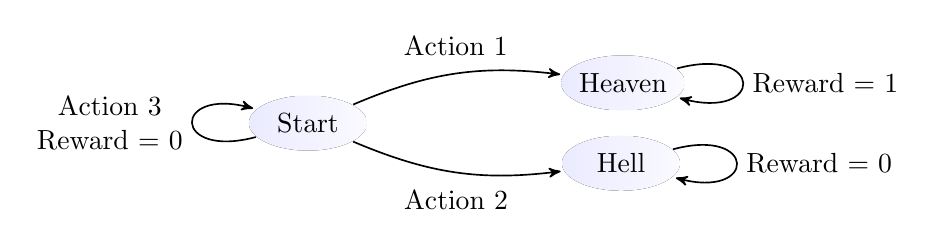
\begin{tikzpicture}[>=stealth', shorten >=1pt, auto, node distance=2.9cm, semithick]
        % Styles for uniform, larger nodes
        \tikzstyle{state} = [ellipse, minimum width=1.5cm,minimum height=.7cm, inner sep=0,path picture={\fill[left color=blue!8, right color=blue!2] (path picture bounding box.south west) rectangle (path picture bounding box.north east);}]

        % States
        \node[state] (S1) {Start};
        \node[state, above right=0cm and 2.9cm of S1] (Heaven) {Heaven};
        \node[state, below right=0cm and 2.9cm of S1] (Hell) {Hell};

        % Arrows
        \path[->] (S1) edge[bend left=15] node[midway, above=.1cm] {Action 1} (Heaven)
                       edge[bend right=15] node[midway, below=.1 cm] {Action 2} (Hell);
        \path[->] (Heaven) edge[loop right] node[right] {Reward = 1} (Heaven);
        \path[->] (S1) edge[loop left] node[left, align=center] {Action 3\\ Reward = 0} (S1);        
        \path[->] (Hell) edge[loop right] node[right] {Reward = 0} (Hell);

    \end{tikzpicture}
    \caption{A variant of \Cref{fig:heaven_hell_problem} which could be called the ``Heaven or Hell or Purgatory'' problem. Now a third action is available which keeps the agent in the starting state and provides reward 0. Action 3 is always safe, as it avoids Hell and retains the option to enter Heaven. However, Action 1 leads to much higher reward and is also safe. This example shows that knowing a safe policy upfront does not resolve the Heaven or Hell problem, since the agent can only obtain high reward if it reaches Heaven, and knowing that Action 3 is safe does not help the agent to determine whether Action 1 or Action 2 will lead to Heaven.}
    \label{fig:purgatory}
\end{figure}


\paragraph{A strictly safe policy is known.} Another option is to assume that a safe policy $\pi_0$ is known upfront \citep{liu2021learning,stradi2024learning}. Not only is this a strong assumption, it is also insufficient: there exist simple instances where $\pi_0$ produces low reward, but the agent has no safe way to explore beyond $\pi_0$ (\Cref{fig:purgatory}). In order to allow the agent to safely explore beyond $\pi_0$, the two references above both also assume a multi-episode setting and assume that $\pi_0$ is ``strictly safe'', i.e., it satisfies the safety constraints with slack.


\subsection{Allowing external help.}

We avoid repeating information from \Cref{sec:related}, so we have just two points we wish to add here. First, we mentioned that \citet{kosoy_delegative_2019} relies on Bayesian inference, but it is worth noting that the majority of papers in this category rely on Bayesian inference \citep{cohen_pessimism_2020, cohen_curiosity_2021, mindermann_active_2018}. These papers also face Bayesian inference's tractability challenges, as discussed in \Cref{sec:related}. To our knowledge, the only prior papers which use external help to obtain safety guarantees without Bayesian inference are \citep{maillard_active_2019,plaut_avoiding_2024}.

Second, several papers which we list under ``focus is safety only'' do include guarantees relating to the agent's reward \citep{cohen_pessimism_2020, cohen_curiosity_2021}. However, those guarantees are of the form ``define regret relative to prior errors'' and thus are subject to the weaknesses discussed previously.

\subsection{Other related work} 

The idea of designing agents which act cautiously when uncertain is not novel. Indeed, this idea is so fundamental that the prior work on this topic far outstrips what we can cover here. Representative theoretical papers include \citet{cortes2018online, hadfield-menell_inverse_2017, li2008knows}. Our model is also reminiscent of active learning \citep{hanneke2014active} due to how the agent proactively requests information and of imitation learning \citep{osa_algorithmic_2018} due to how the agent attempts to imitate the mentor. However, we are not aware of any relevant technical implications. Finally, see \citet{garcia_comprehensive_2015,gu_review_2024, krasowski_provably_2023} for surveys of the safe RL literature.



\section{Comprehensive discussion of \citet{plaut_avoiding_2024}}\label{sec:ac-full}

This section provides technical details relating to \citet{plaut_avoiding_2024} which were omitted from \Cref{sec:ac-overview}. We also reproduce the pseudocode for their Algorithm 1 here for convenience.

\subsection{Comprehensive comparison between our model and that of \citet{plaut_avoiding_2024}}

\Cref{tab:model-comparison-full} provides a complete list of the differences between our models. The first four were already covered in \Cref{sec:ac-overview}, but we discuss the last three here.


\paragraph{Source of next state.} In an MDP, each state is generated by the transition kernel $P$. In the online learning literature (and in \citet{plaut_avoiding_2024}), each state is generated by an adversary as a function of the events of all previous timestamps.\footnote{One can also consider a non-adaptive or ``oblivious'' adversary, but \citet{plaut_avoiding_2024} allow adaptive adversaries.} Clearly an MDP transition kernel is one way for the adversary to choose the next state, so any result which applies to all adversaries also applies to an MDP transition kernel.

\begin{table}[tb]
\centering
\caption{A complete list of differences between our model and that of \cite{plaut_avoiding_2024}. The first four were covered in \Cref{sec:ac-overview}.}
\begin{tabular}{p{0.18\textwidth} p{0.36\textwidth} p{0.36\textwidth}}
\toprule
\textbf{Aspect} & \textbf{Our model} & \textbf{Model of \cite{plaut_avoiding_2024}} \\
\midrule
Conceptual goal & Maximize reward and avoid catastrophe & Avoid catastrophe only \\
% \midrule
% Reward meaning & Typical meaning & Chance of no catastrophe that round\\
\midrule
Objective & Sum of payoffs & Product of payoffs \\
\midrule
Regret definition & Agent and mentor evaluated on $\smols,\sm$ & Agent and mentor both evaluated on $\smols$ \\
\midrule
Desired regret & Sublinear in $T$ & Subconstant in $T$ \\
\midrule
Source of next state & MDP transition kernel & Adversary \\
\midrule
Smoothness & $\sigma$-smooth transition kernel & $\sigma$-smooth adversary \\
\midrule
Agent observations & queries \& possibly rewards & queries only\\
\bottomrule
\end{tabular}
\label{tab:model-comparison-full}
\end{table}


\paragraph{Smoothness.} A $\sigma$-smooth adversary cannot directly pick $s_t$ but must sample $s_t$ from a distribution
$\mathcal{D}_t$ whose concentration is upper-bounded by $1/\sigma$ times the uniform distribution. In an MDP, $s_t$ is sampled from the distribution $P(s_{t-1}, a_{t-1})$, so a $\sigma$-smooth adversary corresponds to a $\sigma$-smooth $P$ as defined in \Cref{sec:model}.

\paragraph{Agent observations.} In most of the online learning literature, the agent observes each reward it obtains. However, \citet{plaut_avoiding_2024} actually do not allow the agent to observe rewards. This is because in their model, each reward represents the chance of catastrophe on the time step. In most scenarios, one only observes whether catastrophe occurred, not its probability. 

In MDPs, typically the agent does observe rewards, since this is the only way for it to learn which states and actions are good. However, observing rewards turns out to be irrelevant for our results. This is because (1) our reduction does not utilize any reward observations and (2) the algorithm from \citet{plaut_avoiding_2024} is assumed to not observe rewards, as mentioned.


\begin{algorithm}[ht!]
\caption{\textit{NovelSelect}}
\label{alg:novelselect}
\begin{algorithmic}[1]
\State \textbf{Input:} Data pool $\mathcal{X}^{all}$, data budget $n$
\State Initialize an empty dataset, $\mathcal{X} \gets \emptyset$
\While{$|\mathcal{X}| < n$}
    \State $x^{new} \gets \arg\max_{x \in \mathcal{X}^{all}} v(x)$
    \State $\mathcal{X} \gets \mathcal{X} \cup \{x^{new}\}$
    \State $\mathcal{X}^{all} \gets \mathcal{X}^{all} \setminus \{x^{new}\}$
\EndWhile
\State \textbf{return} $\mathcal{X}$
\end{algorithmic}
\end{algorithm}


\subsection{Another algorithm from \citet{plaut_avoiding_2024}}

In the main body, we focused on the primary algorithm from \citet{plaut_avoiding_2024} (\Cref{alg:nd}). However, they provide a second algorithm with the same guarantee of subconstant regret under different assumptions.

\begin{lemma}[Theorem D.3 in \citet{plaut_avoiding_2024}]
\label{lem:bucket-regret}
Assume that $\s \subseteq \bbr$ and that $\pi^m(s)$ switches at most $K$ times as $s$ moves from $-\infty$ to $+\infty$. Then for any $c \in (1/2,1)$ Algorithm 4 in \citet{plaut_avoiding_2024} satisfies \Cref{def:ac} with
\begin{align*}
Q_T  \le&\ (\diam(\smols)+4)T^c\\
\rac \le&\  2LKT^{1-2c}
\end{align*}
\end{lemma}

Combining \Cref{lem:bucket-regret} with \Cref{thm:main} produces the following alternative no-regret guarantee:

\begin{theorem}
\label{thm:bucket}
For any $c \in (0,1)$, Algorithm 4 from \citet{plaut_avoiding_2024} satisfies
\begin{align*}
Q_T \le&\ KLT^{2(1-c)}\\
R_T  \le&\ (1+\diam(\smols))T^c
\end{align*}
\end{theorem}

\subsection{Additive vs multiplicative subconstant regret}

See \Cref{sec:ac-overview} for the preliminary discussion of additive vs multiplicative subconstant regret. Here we formalize a connection between these two metrics. Specifically, \Cref{prop:sum-prod} states that when we take the supremum over payoff functions and payoffs are in $[0,1]$, these objectives roughly coincide. This is not an exact equivalence, but the approximation $1+x \approx \exp(x)$ for $x \approx 0$ implies that $1-\exp \big(\sum_{t=1}^T \mu_t(s_t,a_t) -\sum_{t=1}^T \mu_t^m(s_t) \big) \approx  \sum_{t=1}^T \mu_t^m(s_t) - \sum_{t=1}^T \mu_t(s_t, a_t)$ when the latter is small (e.g., the additive regret is subconstant).

\begin{restatable}{proposition}{propSumProd}
\label{prop:sum-prod}
For any MDP $\M$ and mentor policy $\pi^m$, every algorithm satisfies
\begin{align*}
0 \le&\ \sup_{\bfmu}\ \E\left[1-\exp \left(\sum_{t=1}^T \mu_t(s_t,a_t) -\sum_{t=1}^T \mu_t^m(s_t) \right)\right]\\ \le&\ \sup_{\bfmu}\  \E\left[\prod_{t=1}^T \mu_t^m(s_t) - \prod_{t=1}^T \mu_t(s_t, a_t)\right]\\
\le&\ \sup_{\bfmu}\ \E \left[\sum_{t=1}^T \mu_t^m(s_t) - \sum_{t=1}^T \mu_t(s_t, a_t)\right]
\end{align*}
\end{restatable}


We will need the following lemma for the proof:


\begin{lemma}[Lemma B.3 in \citet{plaut_avoiding_2024}]
\label{lem:pos-prod-bound}
Assume $x_1,\dots,x_T, y_1,\dots,y_T \in [0,1]$ and $x_t \ge y_t$ for all $t \in [T]$. Then
\[
\prod_{t=1}^T x_t - \prod_{t=1}^T y_t \le \sum_{t=1}^T x_t - \sum_{t=1}^T y_t
\]
\end{lemma}


\begin{proof}[Proof of \Cref{prop:sum-prod}]
Let $\U$ be the set of payoff functions satisfying $L$-local generalization; then $\mu_t \in \U$ for all $t \in [T]$ and the suprema range over $\bfmu \in \U^T$.

\textbf{Part 1: the first inequality.} Let $\nu_t(s,a) = 0$ for all $s\in \s, a \in \A, t \in [T]$. We have $\nu_t \in \U$ trivially for all $t \in [T]$, so
\[
\sup_{\bfmu}\ \E\left[1-\exp \left(\sum_{t=1}^T \mu_t(s_t,a_t) -\sum_{t=1}^T \mu_t^m(s_t) \right)\right] \ge  \E\left[1-\exp \left(\sum_{t=1}^T \nu_t(s_t,a_t) -\sum_{t=1}^T \nu_t^m(s_t) \right)\right] = 1 - \exp(0) = 0
\]
\textbf{Part 2: the second inequality.} For each $\mu \in \U$, define another payoff function $f(\mu): \s \times \A \to [0,1]$ by $f(\mu)(s,a) = 1 - \mu^m(s) + \min(\mu^m(s), \mu(s,a))$. Let $f(\mu^m)(s) = f(\mu)(s,\pi^m(s))$ for brevity. Note that $\min(\mu^m(s), \mu(s,\pi^m(s))) = \mu^m(s)$ and thus $f(\mu^m)(s) = 1 $ for all $s \in \s$.

We first claim that for all $\mu \in \U$, $f(\mu) \in \U$. For any $s,s' \in \s$, either $f(\mu)(s,\pi^m(s')) = 1 - \mu^m(s) + \mu^m(s) = 1$, or $f(\mu)(s,\pi^m(s')) = 1 - \mu^m(s) + \mu(s,\pi^m(s'))$. In the former case, we have
\[
|f(\mu^m)(s) - f(\mu)(s,\pi^m(s'))| = |1-1| = 0 \le L \norm{s-s'}
\]
and in the latter case, we have
\begin{align*}
|f(\mu^m)(s) - f(\mu)(s,\pi^m(s'))| =&\ |1 - (1 - \mu^m(s) + \mu(s, \pi^m(s')))|\\
=&\ |\mu^m(s) - \mu(s,\pi^m(s'))|\\
\le&\ L\norm{s-s'}
\end{align*}
with the last step due to $\mu \in \U$. Therefore $f(\mu) \in \U$. Now fix any $s_1,\dots,s_T$ and $a_1,\dots,a_T$. Using the standard inequality $\log(1+x) \le x$ for all $x \in \bbr$,
\begin{align*}
\prod_{t=1}^T f(\mu_t)(s_t, a_t) =&\ \exp \sum_{t=1}^T \log \big(f(\mu_t)(s_t, a_t)\big)\\
=&\ \exp \sum_{t=1}^T \log \big(1 - \mu_t^m(s_t) + \min(\mu_t^m(s_t), \mu_t(s_t,a_t))\big)\\
\le&\ \exp \sum_{t=1}^T \big(- \mu_t^m(s_t) + \min(\mu_t^m(s_t), \mu_t(s_t,a_t))\big)\\
=&\ \exp \left(\sum_{t=1}^T \min(\mu_t^m(s_t), \mu_t(s_t,a_t)) -\sum_{t=1}^T \mu_t^m(s_t) \right)\\
\le&\ \exp \left(\sum_{t=1}^T  \mu_t(s_t,a_t) -\sum_{t=1}^T \mu_t^m(s_t) \right)
% \le&\ \exp \left(\sum_{t=1}^T \mu_t(s_t,a_t) -\sum_{t=1}^T \mu_t^m(s_t) \right)
\end{align*}
Since this holds for any $s_1,\dots,s_T$ and $a_1,\dots,a_T$, we have
\[
\E\left[\prod_{t=1}^T f(\mu_t)(s_t, a_t)\right] \le \E\left[\exp \left(\sum_{t=1}^T  \mu_t(s_t,a_t) -\sum_{t=1}^T \mu_t^m(s_t) \right)\right]
\]
Let $\U_f$ be the image of $\U$ under $f$, i.e., $\mu \in \U_f$ if there exists $\mu' \in \U$ such that $f(\mu') = \mu$. Then $(f(\mu_1),\dots,f(\mu_T)) \in \U_f^T$. Since $f(\mu) \in \U$ for all $\mu \in \U$, we have $\U_f \subseteq \U$, and thus $\U_f^T \subseteq \U^T$. Therefore
\begin{align*}
\sup_{\bfmu \in \U^T}  \E\left[\prod_{t=1}^T \mu_t^m(s_t) - \prod_{t=1}^T \mu_t(s_t, a_t)\right] \ge&\ \sup_{\bfmu \in \U_f^T}  \E\left[\prod_{t=1}^T \mu_t^m(s_t) - \prod_{t=1}^T \mu_t(s_t, a_t)\right]\\
=&\ \sup_{\bfmu \in \U^T} \E\left[\prod_{t=1}^T f(\mu_t^m)(s_t) - \prod_{t=1}^T f(\mu_t)(s_t, a_t)\right]\\
\ge&\ \sup_{\bfmu \in \U^T} \E\left[1 - \exp \left(\sum_{t=1}^T \mu_t(s_t,a_t) -\sum_{t=1}^T \mu_t^m(s_t) \right)\right]
\end{align*}
\textbf{Part 3: the third inequality.} The analysis proceeds similarly, but instead of $f(\mu)(s,a)$, we use $g(\mu)(s,a) = \min(\mu^m(s), \mu(s,a))$. Let $g(\mu^m)(s) = g(\mu)(s,\pi^m(s))$ for brevity and note that $g(\mu^m)(s) = \min(\mu^m(s), \mu(s,\pi^m(s))) = \mu^m(s)$ for all $s \in \s$.

For any $s,s' \in \s$, either $g(\mu)(s,\pi^m(s')) = \mu^m(s)$ or $g(\mu)(s,\pi^m(s')) = \mu(s,\pi^m(s'))$. In the former case, 
\[
|g(\mu^m)(s) - g(\mu)(s,\pi^m(s'))| |\mu^m(s) - \mu^m(s)| = 0 \le L\norm{s-s'}
\]
and in the latter case,
\begin{align*}
|g(\mu^m)(s) - g(\mu)(s,\pi^m(s'))| = |\mu^m(s) - \mu(s,\pi^m(s'))| \le L\norm{s-s'}
\end{align*}
with the last step due to $\mu \in \U$. Thus $g(\mu) \in \U$. Let $\U_g$ be the image of $\U$ under $g$; then $\U_g \subseteq \U$ and $\U_g^T \subseteq \U^T$. Since $\mu_t(s_t,a_t) \ge \min(\mu_t^m(s_t), \mu_t(s_t,a_t))$ for all $t \in [T]$, we have $\prod_{t=1}^T \mu_t(s_t,a_t) \ge \prod_{t=1}^T \min(\mu_t^m(s_t), \mu_t(s_t,a_t))$. Also applying \Cref{lem:pos-prod-bound} with $x_t = \mu_t^m(s_t)$ and $y_t = \min(\mu_t^m(s_t), \mu_t(s_t,a_t))$ gives us
\begin{align*}
\E\left[\prod_{t=1}^T \mu_t^m(s_t) - \prod_{t=1}^T \mu_t(s_t, a_t)\right] \le&\ \E\left[\prod_{t=1}^T \mu_t^m(s_t) - \prod_{t=1}^T \min(\mu_t^m(s_t), \mu_t(s_t,a_t))\right]\\
\le&\ \E\left[\sum_{t=1}^T \mu_t^m(s_t) - \sum_{t=1}^T \min(\mu_t^m(s_t), \mu_t(s_t,a_t))\right]
\end{align*}
Therefore
\begin{align*}
\sup_{ \bfmu \in \U^T}  \E\left[\prod_{t=1}^T \mu_t^m(s_t) - \prod_{t=1}^T \mu_t(s_t, a_t)\right] \le&\ \sup_{ \bfmu \in \U^T}  \E\left[\sum_{t=1}^T \mu_t^m(s_t) - \sum_{t=1}^T \min(\mu_t^m(s), \mu_t(s_t, a_t))\right]\\
=&\ \sup_{ \bfmu \in \U^T}  \E\left[\sum_{t=1}^T g(\mu_t^m)(s_t) - \sum_{t=1}^T g(\mu_t)(s_t, a_t)\right]\\
=&\ \sup_{ \bfmu \in \U_g^T}  \E\left[\sum_{t=1}^T \mu_t^m(s_t) - \sum_{t=1}^T \mu_t(s_t, a_t)\right]\\
\le&\ \sup_{ \bfmu \in \U^T}  \E\left[\sum_{t=1}^T \mu_t^m(s_t) - \sum_{t=1}^T \mu_t(s_t, a_t)\right]\\
\end{align*}
as required.
\end{proof}

\section{Proof of \Cref{thm:main}}\label{sec:main-proof}

In \Cref{sec:main}, we stated our main result and provided a proof sketch. Here we provide the formal proof.

Recall the following definitions:
\begin{itemize}
    \item $N_t(s, X) = \Pr[s_{t+1} \in X \mid s_t = s]$
    \item $N_t^m(s, X) = \Pr[s_{t+1}^m \in X \mid s_t^m = s]$
    \item $\alpha_t(X) = \E[N_t^m(s_t, X) - N_t(s_t, X)]$ 
    \item $\Delta_t = \sup_{X\subseteq \s} (p_t^m(X) - p_t(X))$
\end{itemize}

We refer the reader to Chapter 8 of \citet{bertsekas1996stochastic} for a thorough measure-theoretic treatment of MDP theory. In particular, we will not rehash why the assumptions in \Cref{sec:model} are sufficient to ensure that all random variables and expectations are well-defined. However, it is worth proving that $N_t$ and $N_t^m$ are measurable (and thus that $\alpha_t$ is well-defined), since these are not standard functions. Readers unconcerned with measure theory can safely skip \Cref{prop:measure}.

% Before beginning the main proof, we take a moment to ensure that all of the probabilities and expectations we analyze throughout the proof are well-defined. We have tried to strike a balance of covering the measure-theoretic essentials without reinventing the entirety of measure-theoretic MDP theory. Readers unconcerned with measure theory can safely skip \Cref{prop:measure}, while readers who want more details should refer to Chapter 8 of \citet{bertsekas1996stochastic}.

\begin{proposition}
\label{prop:measure}
% For each $t \in [T]$, the random variables $s_t,a_t,q_t$, and $s_t^m$ are well-defined. 
For any fixed $X\subseteq\s$ and any $t \in [T]$, the functions $N_t(\cdot,X) \to [0,1]$ and $N_t^m(\cdot, X) \to [0,1]$ are measurable on $\s$.
\end{proposition}

\begin{proof}
% We show inductively that $s_t,a_t,q_t$, and $s_t^m$ are well-defined. The initial state $s_1 = s_1^m$ is fixed. Suppose that the agent's history $h_t = s_1,a_1,q_1,\dots,s_t$ and the mentor's history $h_t^m = s_1^m,\pi^m(s_1^m),\dots,s_t^m$ are well-defined random variables. By assumption, the agent's choices of $a_t,q_t$ and the mentor's action policy $\pi^m$ are measurable functions of the history,\footnote{In the mentor's case, $\pi^m$ only depends on $s_t^m$, but the statement still holds.} so $a_t,q_t$ and $\pi^m(s_t)$ are well-defined. Since $s_t, a_t, s_t^m,$ and $\pi^m(s_t)$ are well-defined and $P$ is a transition kernel, $s_{t+1}$ and $s_{t+1}^m$ are also well-defined. Thus $h_{t+1} = h_t, a_t,q_t,s_{t+1}$ and $h_{t+1}^m = h_t^m, \pi^m(s_t^m), s_{t+1}^m$ are well-defined, which completes the induction. We conclude that $s_t,a_t,q_t$, and $s_t^m$ are well-defined random variables.

Let $\D(a_t)$ denote the distribution of the random variable $a_t$. By the law of total expectation,
\begin{align*}
N_t(s,X) =&\ \Pr[s_{t+1} \in X \mid s_t = s]\\
=&\ \E_{a \sim \D(a_t)}\big[\E[\bfone(s_{t+1} \in X) \mid s_t = s, a_t=a]\big]\\
=&\ \E_{a \sim \D(a_t)} \big[\E[P(s,a,X)]\big]\\
=&\ \E[P(s,a_t,X)]
\end{align*}
Since $P(\cdot,\cdot,X)$ is measurable, the expectation $\E[P(s,a_t,X)]$ is well-defined and is itself a measurable function on $\s$. Therefore $N_t(\cdot,X) = \E[P(\cdot,a_t,X)]$ is measurable on $\s$.

Since the mentor's action in state $s$ is deterministically $\pi^m(s)$, we have $N_t^m(s, X)= P(s,\pi^m(s),X)$. Thus $N_t^m(\cdot,X)$ is the composition of measurable functions $P(\cdot,\cdot,X)$ and $\pi^m$, so $N_t^m(\cdot,X)$ is also measurable.
\end{proof}

We now proceed to the main proof.

\lemSplit*

\begin{proof}
By the tail sum formula for expected value (see, e.g., Lemma 4.4 in \citet{kallenberg1997foundations}), we have
\begin{align*}
\E[f(s_t^m)] =&\ \int_{h=0}^\infty \Pr[f(s_t^m) > h] \d h\\
\E[f(s_t)] =&\ \int_{h=0}^\infty \Pr[f(s_t) > h] \d h
\end{align*}
Since $f(s) \in [0,1]$ for all $s \in \s$, we can restrict the integrals to $[0,1]$. Next, for each $h \in \bbrpos$, define $X_h = \{s \in \s: f(s) > h\}$. Each $X_h$ is measurable since it is the preimage of a measurable function $f$ on the open set $(h, \infty)$. Therefore
\begin{align*}
\Pr[f(s_t^m) > h] =&\ \Pr[s_t^m \in X_h] = p_t^m(X_h)\\
\Pr[f(s_t) > h] =&\ \Pr[s_t \in X_h] = p_t(X_h)
\end{align*}
and so
\begin{align*}
\E[f(s_t^m) - f(s_t)] =&\ \int_{h=0}^1 \big(\Pr[f(s_t^m) > h] - \Pr[f(s_t) > h]\big) \d h\\
=&\ \int_{h=0}^1 \big(p_t^m(X_h) - p_t(X_h)\big) \d h\\
\le&\ \int_{h=0}^1 \Delta_t \d h\\
=&\ \Delta_t
\end{align*}
\end{proof}


\lemTrajInd*

\begin{proof}
We proceed by induction. Since the agent and mentor have the same initial state, we have $p_1(X) = p_1^m(X)$ for all $X \subseteq \s$, so $\Delta_1 = 0 = \sum_{i=1}^0 \sup_{X\subseteq\s} \alpha_i(X)$. Thus the lemma holds for $t=1$, so assume the lemma holds for some $t \in [T]$.

Fix any $X \subseteq \s$. The next step is to analyze $\E[N_t(s_t, X)]$, which requires a bit of care since $\E[N_t(s_t, X)]$ is an expectation over $s_t$ but $s_t$ also appears in the definition of $N_t(s,X)$. To prevent confusion, we can rewrite $\E[N_t(s_t, X)]$ as $\E_{s\sim p_t} [N_t(s, X)]$, where $s \sim p_t$ indicates that $s$ is sampled from the same distribution as $s_t$. Then
\begin{align*}
\E[N_t(s_t, X)] =&\ \E_{s \sim p_t}[N_t(s, X)]\\
=&\ \E_{s \sim p_t}[\Pr[s_{t+1} \in X \mid s_t = s]] \\
=&\ \E_{s \sim p_t} \left[\E[\bfone(s_{t+1} \in X) \mid s_t = s]\right] 
\end{align*}
By the law of total expectation,
\[
\E_{s \sim p_t} \E[\bfone(s_{t+1} \in X) \mid s_t = s]] = \E[\bfone(s_{t+1} \in X)] = \Pr[s_{t+1} \in X]
\]
Therefore $\E[N_t(s_t, X)] = p_{t+1}(X)$. The same argument can be used to show that $\E[N_t^m(s_t^m, X)] = p_{t+1}^m(X)$ by simply replacing $s_t$ and $p_t$ with $s_t^m$ and $p_t^m$ respectively. Thus
\begin{align*}
p_{t+1}^m(X) - p_{t+1}(X) =&\ \E[N_t^m(s_t^m, X)] - \E[N_t(s_t, X)]\\
=&\ \E[N_t^m(s_t^m, X) - N_t^m(s_t, X)] + \E[N_t^m(s_t, X) - N_t(s_t, X)]\\
=&\ \E[N_t^m(s_t^m, X) - N_t^m(s_t, X)] + \alpha_t(X)
\end{align*}
Next, define $f:\s \to[0,1]$ by $f(s) = N_t^m(s,X)$. \Cref{prop:measure} implies that $f$ is measurable, so \Cref{lem:split} implies that $\E[N_t^m(s_t^m,X) - N_t^m(s_t, X)] \le \Delta_t$, which gives us $p_{t+1}^m(X) - p_{t+1}(X) \le \Delta_t + \alpha_t(X) \le \Delta_t + \sup_{Y\subseteq \s} \alpha_t(Y)$. Since this holds for all $X \subseteq \s$, we have 
\[
\Delta_{t+1} = \sup_{X\subseteq \s} (p_{t+1}^m(X) - p_{t+1}(X)) \le \Delta_t + \sup_{X\subseteq \s} \alpha_t(X)
\]
Combining this with the inductive hypothesis of $\Delta_t \le \sum_{i=1}^{t-1} \sup_{X \subseteq \s} \alpha_i(X)$ gives us
\[
\Delta_{t+1} \le \Delta_t + \sup_{X\subseteq \s} \alpha_t(X) \le \sum_{i=1}^t \sup_{X\subseteq \s} \alpha_t(X)
\]
which completes the induction.
\end{proof}

\lemTraj*

\begin{proof}
Fix an arbitrary sequence of subsets $X_1,\dots,X_{t-1} \subseteq \s$ and define $\bfmu$ as follows:
\[
\mu_i(s,a) =
\begin{cases}
P(s,a,X_i) & \text{ if } i \in [t-1]\\
1 & \text{ otherwise}
\end{cases}
\]
For $i > t-1$ we have $|\mu_i(s, \pi^m(s)) - \mu_i(s, \pi^m(s'))| = 0 \le L\norm{s - s'}$. For for $i \in [t-1]$, local generalization of $P$ implies that
\begin{align*}
|\mu_i(s, \pi^m(s)) - \mu_i(s, \pi^m(s'))| =&\ \big|P\big(s,\pi^m(s), X_i)\big) - P(s,\pi^m(s'),X_i)\big)\big|\\
\le&\ \sup_{V \subseteq \s}\big|P\big(s,\pi^m(s), V\big) - P(s,\pi^m(s'),V)\big)\big|\\
=&\ \tv{P(s, \pi^m(s)) - P(s, \pi^m(s'))}\\
\le&\ L \norm{s-s'}
\end{align*}
Therefore $\bfmu$ satisfies local generalization. Next, we analyze $\mu(s_i, a_i)$. As in the proof of \Cref{lem:trajectories-induction}, let $s \sim p_i$ denote sampling $s$ from the same distribution as $s_i$. Also let $\D(a_i)$ denote the distribution of $a_i$. Then for each $i \in [t-1]$,
\begin{align*}
\E[\mu_i(s_i, a_i)] =&\ \E_{s\sim p_i, a\sim \D(a_i)}[\mu_i(s, a)]\\
=&\ \E_{s\sim p_i, a\sim \D(a_i)}[P(s,a,X_i)] && (\text{Definition of $\mu_i$ for $i \in [t-1]$})\\
=&\ \E_{s\sim p_i, a\sim \D(a_i)}[\Pr[s_{i+1} \in X_i \mid s_i = s, a_i = a]] && (\text{Definition of $P(s,a,X_i)$})\\
=&\ \E_{s\sim p_i, a\sim \D(a_i)}[\E[\bfone(s_{i+1} \in X_i) \mid s_i = s, a_i = a]] && (\text{Expectation of indicator variable})\\
=&\ \E[\bfone(s_{i+1} \in X_i)] && (\text{Law of total expectation})\\
=&\ \E[N_i(s_i, X_i)] && (\text{Proof of \Cref{lem:trajectories-induction}})
\end{align*}
Similarly but more simply,
\begin{align*}
N_i^m(s_i,X_i)=&\ \Pr[s_{i+1}^m \in X_i \mid s_i^m = s_i]\\
=&\ P(s_i, \pi^m(s_i), X_i)]\\
=&\ \mu_i(s_i, \pi^m(s_i))
\end{align*}
Therefore
\begin{align*}
\sum_{i=1}^{t-1} \alpha_i(X_i) =&\ \sum_{i=1}^{t-1} \E\left[N_i^m(s_i, X_i) - N_i(s_i, X_i)\right]\\
=&\ \sum_{i=1}^{t-1} \E[\mu_i(s_i, \pi^m(s_i)) - \mu_i(s_i, a_i)]\\
% =&\ \sum_{i=1}^{t-1} \E[\mu_i(s_i, \pi^m(s_i)) - \mu_i(s_i, a_i)] + \sum_{i=t}^T \E[\mu_i(s_i, \pi^m(s_i)) - \mu_i(s_i, a_i)]\\
=&\ \sum_{i=1}^T \E[\mu_i(s_i, \pi^m(s_i)) - \mu_i(s_i, a_i)]\\
\le&\ \sup_{\M, \pi^m, \bfmu}\ \sum_{i=1}^T \E[\mu_i(s_i, \pi^m(s_i)) - \mu_i(s_i, a_i)]\\
=&\ \rac
\end{align*}
Since this holds for any sequence of subsets $X_1,\dots,X_{t-1} \subseteq \s$, we have
\begin{align*}
\sum_{i=1}^{t-1} \sup_{X\subseteq\s} \alpha_i(X)= \sup_{X_1,\dots,X_{t-1} \subseteq \s} \sum_{i=1}^{t-1} \alpha_i(X_i) \le \rac
\end{align*}
Applying \Cref{lem:trajectories-induction} completes the proof.
\end{proof}

\thmMain*

\begin{proof}
The query bound follows trivially from \Cref{def:ac}, so we proceed to the regret bound. Let $r^m(s) = r(s, \pi^m(s))$ for brevity. Then $r^m: \s \to [0,1]$ is the composition of measurable functions $r$ and $\pi^m$, so $r^m$ is also measurable. Hence \Cref{lem:split} implies that $\E[r^m(s_t^m) - r^m(s_t)] \le \Delta_t$ for all $t \in [T]$. Therefore
\begin{align*}
\E\left[r^m(s_t^m) - r(s_t, a_t)\right] =&\ \E[r^m(s_t^m) - r^m(s_t)] + \E[r^m(s_t) - r(s_t, a_t)]\\
\le&\ \Delta_t +\E[r^m(s_t) - r(s_t, a_t)]
\end{align*}
Lemmas~\ref{lem:action-regret} and \ref{lem:trajectories} respectively imply that $\E \big[\sum_{t=1}^T r^m(s_t) - r(s_t, a_t)\big] \le  \rac$ and $\Delta_t \le \rac$, so\looseness=-1
\begin{align*}
R_T =&\ \E\left[\sum_{t=1}^T r^m(s_t^m) - \sum_{t=1}^T r(s_t, a_t)\right]\\
\le&\ \sum_{t=1}^T \Delta_t +\E \left[\sum_{t=1}^T r^m(s_t) - r(s_t, a_t)\right]\\
\le&\ T \rac +\rac\\
\le&\ (T+1) \rac
\end{align*}
as required.
\end{proof}

\subsection{Less general proof without assuming local generalization for $r$}\label{sec:alt}

In case the of Algorithm 1, we can avoid assuming local generalization for $r$ by using the following result from \citet{plaut_avoiding_2024}, where $M_T = \{t \in [T]: a_t \ne \pi^m(s_t)\}$:

\begin{lemma}[Lemma B.1 in \citet{plaut_avoiding_2024}]
Under the conditions of \Cref{lem:ac-regret}, $\E[|M_T|] \in O(\frac{d}{\sigma} T^\frac{1}{2n+1} \log T)$.
\end{lemma}

Two minor differences exist between the version of Lemma B.1 in \citet{plaut_avoiding_2024} and what we have stated above:
\begin{enumerate}
    \item Lemma B.1 in \citet{plaut_avoiding_2024} is in terms of $\ep$; we have again plugged in $\ep = T^\frac{-2n}{2n+1}$, as discussed above. 
    \item In \citet{plaut_avoiding_2024}, $M_T$ is actually defined as $\{t \in [T]: \pi_t(s_t) \ne \pi^m(s_t)\}$, where $\pi_t(s_t)$ is an action proposed by the algorithm, and the algorithm ends up either taking action $\pi_t(s_t)$ or querying. Clearly if the agent queries then $a_t = \pi^m(s_t)$, so $\{t \in [T]: a_t \ne \pi^m(s_t)\} \subseteq \{t \in [T]: \pi_t(s_t) \ne \pi^m(s_t)\}$. Thus their bound from Lemma B.1 also applies to our slightly more restrictive definition of $M_T$.
\end{enumerate}

\begin{theorem}
\label{thm:no-lg}
Assume $P$ satisfies local generalization, but $r$ does not. Under the conditions of \Cref{lem:ac-regret}, Algorithm 1 from \citet{plaut_avoiding_2024} satisfies $Q_T \in o(T)$ and $R_T \in o(T)$.
\end{theorem}

\begin{proof}
We perform the same analysis as in the original proof to reach $\E[\sum_{t=1}^Tr(s_t^m, \pi^m(s_t^m)) - \sum_{t=1}^T r(s_t, a_t)] \le \sum_{t=1}^T \Delta_t+\E [\sum_{t=1}^T r(s_t, \pi^m(s_t)) - r(s_t, a_t)]$. As before, we use \Cref{lem:trajectories} to show that $\sum_{t=1}^T \Delta_t \le T\rac$, which requires $P$ to satisfy local generalization. Previously, we bounded $\E [\sum_{t=1}^T r(s_t, \pi^m(s_t)) - r(s_t, a_t)]$ by applying \Cref{def:ac} to $\mu_t(s,a) = r(s,a)$, which requires $r$ to satisfy local generalization. Here, we instead note that $r(s_t, \pi^m(s_t)) > r(s_t, a_t)$ can only occur when $a_t \ne \pi^m(s_t)$. Therefore
\begin{align*}
\E \left[\sum_{t=1}^T r(s_t, \pi^m(s_t)) -\sum_{t=1}^T r(s_t, a_t)\right] \le&\ \E \left[\sum_{t \in M_T} (r(s_t, \pi^m(s_t)) - r(s_t, a_t))\right]\\
\le&\ \E \left[\sum_{t \in M_T} 1\right]\\
=&\ \E \left[|M_T|\right]\\
\in&\ O\left(\frac{d}{\sigma} T^\frac{1}{2n+1} \log T\right)
\end{align*}
\Cref{lem:ac-regret} implies that $\rac \in O(\frac{dL}{\sigma} T^\frac{1}{2n+1} \log T)$, so we conclude that
\begin{align*}
R_T \le&\ T \cdot O\left(\frac{dL}{\sigma} T^\frac{1}{2n+1} \log T\right) + O\left(\frac{d}{\sigma} T^\frac{1}{2n+1} \log T\right)\\
\in&\ O\left(\frac{dL}{\sigma} T^\frac{2n}{2n+1} \log T\right)
\end{align*}
We conclude that $R_T \in o(T)$.
\end{proof}


\end{document}
